%!TEX root = vaisagh_thesis.tex

\chapter{A Game-based Investigation into the Role of Memory in Human Exploration and Navigation}
\label{chapter:SpatialKnowledgeChapter}
\chaptermark{Investigating the effect of memory on Indoor Wayfinding}

Several studies have shown that during egress people tend to take routes that are familiar to them rather than the shortest route~\cite{Mawson:2005tq,Paulsen:1984ti,Ramachandran:1990wj,Sandberg:1997tw}. This is because, in most cases, occupants of a building do not have a complete cognitive map of its layout. This is sometimes the case even after the occupants work in the building for several months~\cite{Moeser01011988}. However, existing agent based models of egress, generally make the simplifying assumption that occupants have complete knowledge of the environment. In the rare cases like~\cite{Pelechano:2006ba} where partial knowledge is modeled, it is simply assumed that people have an eidetic memory and never forget a room that they perceive once. Moreover, it is arbitrarily assumed that agents explore unknown environments in either a depth first or a breadth first manner. How people explore unknown environments and gain spatial knowledge from this will obviously have an impact on the paths that are taken during egress. However, a major difficulty in modelling spatial knowledge accurately is our limited understanding of the role of memory in indoor wayfinding and exploration. In this chapter, we try to address this issue.






% THe problem we want to solve
How humans gain and store knowledge of their surroundings has been an area of research for several decades now~\cite{lynch_image_1960,Thorndyke1982560,Kuipers78,Siegel19759,Kuipers01012003}. A significant amount of research has been conducted in trying to understand how wayfinding is done using this knowledge in outdoor environments~\cite{Kuipers78,Gopal1989309}. However, there has been much less work done on indoor exploration~\cite{Kuipers01012003,HolscherBMS06,stankiewicz2006lost,stankiewicz2007acquistion}. With the increasing number of shopping malls, airports, high rise office buildings and residential towers, there is an increasing likelihood that the occupants of a building may not be regular visitors and as a result will have very little knowledge of the layout. If in such a situation, there is a need to evacuate the building, it is important for planners to know how the occupants would react and find their way to the emergency exits. However, there are several aspects of how people explore an unfamiliar environment and the interaction between exploration and memory during this process that is still not understood. More importantly, we believe that existing methods for studying this interaction are limited in certain ways.

% LImitations of most existing work
Understanding how people navigate and explore unknown spaces is scientifically challenging. One of the primary reasons is that experimentally studying such processes  is difficult and time consuming. Even after an experiment is designed, it is often difficult to scale the experiments to many participants and therefore account for various forms of sampling bias. This can be seen in several existing studies like~\cite{Kuipers01012003,stankiewicz2006lost,stankiewicz2007acquistion} which, despite having experiments that are excellently designed, suffer from having few participants and thus probably being susceptible to sampling bias.

% Possible solutions
%mhl - add more references, try to find good ones from psychology
Recently, Bode and Codling~\cite{Bode2013347} demonstrated a possible solution to this problem by using a point and click game to study exit route choice during evacuation and getting more than 150 participants to participate in their experiment. Recent years have seen the emergence of serious games (or gamification) as an approach for conducting human subject experiments~\cite{Anonymous:2011ba,Aydt:2011wz,Michael:2005:SGG:1051239,Waller:2002we}. This approach can elicit the same behavioral response as real world experiments~\cite{Montello:2004uj} while reducing the overhead associated with conducting large-scale real world experiments. In the past this type of approach has been used for validating crowd simulation models~\cite{npelechano:2008ug, Anonymous:2011ba, Viswanathan2014} and understanding behavioral responses to dynamic information during egress~\cite{Bode06022014,Viswanathan:ut}. Serious games~\cite{Michael:2005:SGG:1051239} have a long history in training, for example, aircraft simulation~\cite{hays1992flight} and medical training~\cite{jama.282.9.861}.

%In this chapter games are used only to observe the participant behaviors, whereas for training, the objective is both to observe and steer behavior.

Due to the nature of the data under consideration, namely spatio-temporal tracks of many individuals, \emph{desktop virtual reality experiments} are the most practical way to conduct such experiments~\cite{stankiewicz2006lost,stankiewicz2007acquistion}. For exploration in particular, the use of a virtual environment allows the experimenter to design particular structures and understand how they affect people's decisions. We believe that packaging the experiment in a game, rather than as a standard social experiment, is an ideal way to scale to large sample sizes.

In this chapter we adopt the same methodology to gain an understanding of how humans, with no knowledge of an environment, explore. The method involves experiments in which participants play an exploration game; in the game, they are asked to explore a multi-floor building and complete a set of tasks within a certain time limit. All the movement and actions of the players are logged and later analyzed for patterns. We then propose a novel way of identifying the role that memory and {\em non-randomness} plays in human exploration from the data extracted.
Thus, the main motivations of this chapter, and therefore its main contributions, are :
\begin{enumerate}
\item The development of a novel and scalable game based methodology to study indoor wayfinding behavior.
\item The demonstration of such a scalable method's usefulness in determining how memory influences exploration efficiency and an individual's ability to navigate within an environment.
\end{enumerate}

The remainder of this chapter is organized as follows: Section~\ref{sec:literature_review} first provides an overview of our current understanding of how people gain spatial knowledge and do indoor wayfinding. Following this, the game and experiment are described in Section~\ref{sec:experiment_performed_minecraft}. The methodology used for evaluating the results from the grame are then explained in Section~\ref{sec:methodologies}. Finally, the results and its implications are discussed in Section~\ref{sec:analysis_of_experiment_results}.\footnote{This chapter has been submitted to Nature Scientific Reports for review.}

\section{Literature Review} % (fold)
\label{sec:literature_review}

% Bo An: This section is a bit loose. Rather than just listing some related work, you may also discuss their limitation and say something about how your approach overcomes their limitations.

Human exploration of indoor environments is a complex process that may depend on many factors including the perception of the environment, the person's existing knowledge and various cultural factors. Before examining existing models of human exploration it is useful to establish a basic knowledge of how spatial knowledge is stored, used and updated in human memory. In the context of this chapter, it is also useful to understand the methodology used in studying human spatial memory as both an inspiration and validation for the methodology adopted here.

\subsection{Working memory} % (fold)
\label{sec:spatial_information_in_human_working_memory}


Since Hebb's work on human memory~\cite{DOH1949}, it has generally been accepted that human memory has a Short Term Memory (STM) component and a Long Term Memory (LTM) component. Baddeley's model of working memory~\cite{BaddeleyHitch74}, which is a three component model consisting of the central executive, a visual spatial sketchpad and a phonological loop is currently one of the most popular models of the working of human memory. Central to this idea is the concept of \emph{working memory}. Working memory consists of both a visual and a verbal component both of which are limited in capacity.


In order to study the use of memory during wayfinding, Lindberg and G{\"a}rling~\cite{lindberg1981acquisition} presented people with a difficult task to complete (backward counting), while concurrently performing wayfinding. They discovered that the concurrent task adversely affected wayfinding performance. This supported the notion that navigation may require effective use of limited capacity cognitive sub-systems. However, the relative involvement of different cognitive sub-systems could not be determined through this experiment. Several studies~\cite{Garden1992, meilinger2008working} have involved experiments examining the way in which wayfinding memory is stored. These studies concluded that when maps were used for learning, only the visuo-spatial component of memory was used. However, in the real world, they found that all the senses were used together and that verbal, visuo-spatial, temporal, auditory and even olfactory cues were used by the participants. This supports the notion that experiments studying wayfinding without maps should be as immersive as possible to ensure they reflect reality.

Evidence suggests that salient (distinctive) cues are important for place learning. This is especially true as people age and reduce their ability to perceive and process cues~\cite{Davis01122009} or if the way-finders are stressed or under time pressure~\cite{Ozel:2001tn}. This is quite probably due to the fact that both stress and old age can reduce working memory capacity. A decreased working memory capacity implies a smaller amount of environmental information is processed and less information is eventually encoded. This, in turn, implies that only cues that have high perceptual, cognitive or contextual salience are perceived~\cite{Davis01122009} in stressful situations like emergency evacuations that are the main subject of this thesis.

In summary, human working memory consists of different components for processing different types of cues. Experiments show that different cues are used during wayfinding and thus an experiment to study this behavior should be as \emph{immersive} as possible. Also, wayfinding behavior is likely to be different in stressful scenarios due to cognitive constraints in cue processing. Thus, recreation of a stress or time pressure is necessary to recreate egress wayfinding behavior in experiments.

\subsection{The building blocks of spatial knowledge} % (fold)
\label{sub:how_people_gain_spatial_information}

There are different {\em scales} at which locations are stored in the human mind. According to Sholl and Fraone~\cite{Sholl:2004vu}, these can broadly be divided into 3 levels: Figural Spaces (Object Sized Space), Room Sized Space (Vista Sized Space), Environment Space (Map Sized Space). The accepted approaches and methodologies employed to study and understand these different scales depend on the scale concerned~\cite{Sholl:2004vu}. In this research, we specifically consider Vista and Map sized spaces.

One of the earliest and most influential works on how humans gain and store knowledge of space was Lynch's \emph{The Image of the City}~\cite{lynch_image_1960}. He coined the term \emph{mental map} which refers to a person's perception of the world around him. Perhaps the most important contribution of Lynch's paper was the proposal of the fundamental building blocks of a mental map: paths, edges, districts, nodes and landmarks. Paths are routes along which people move, districts are distinct regions, edges define the boundaries between these regions, nodes and landmarks are locations that are points of reference in the mental maps.

How these blocks form a person's image of space was explored by Siegel and White~\cite{Siegel19759} through their experiments on map learning in children. They proposed a hierarchical model with three distinct parts. They found that people first gain knowledge of the \emph{landmarks} in an area, subsequently they learn \emph{routes} connecting these landmarks and finally they gain \emph{survey knowledge}, wherein they have an overall map of the region to the extent that they can determine shortcuts and best routes. They further postulated that adults, despite having more developed cognitive abilities than a child, mirror a similar process in forming their memory of space.

 Ishikawa and Montello~\cite{Ishikawa200693} emphasized that different people have different abilities and techniques for formation of spatial knowledge. Significantly, they found that given repeated exposure to the environment, some people were inherently good and others inherently bad at forming and using spatial knowledge.

 Some researchers~\cite{Moeser01011988,Ishikawa200693} argue that, contrary to Siegel and White, people's route knowledge and knowledge of space does not significantly improve after first being formed. More interestingly they discovered that certain routes are learned and these routes do not change much; however, inter route connections improve as experience increases.

 In summary, while people do have different techniques of forming and storing spatial knowledge, most studies have confirmed that there is a definite pattern in which it is formed, with landmarks and routes playing a key role at the beginning. Furthermore, studies have also shown that this initial knowledge of routes does not change much with time. This implies that the way in which people first explore an environment most likely plays a key role in determining the route they learn and use. This clearly indicates the crucial role that exploration plays in both short-term and long-term way finding behaviour, thus motivating the need for a better understanding of the way in which humans explore environments.

% subsection the_pioneering_work (end)
\subsection{Wayfinding in indoor environments} % (fold)
\label{sec:indoor_wayfinding}

Literature on human behavior in internal environments, in general, is much more limited than on outdoor wayfinding. \cite{best1970direction} was the first to identify that the number of choice points, that is, locations where directional changes occurred, was the relevant measure for assessing way finding difficulty, as opposed to simple metric distances.


\cite{Weisman01031981} defined visual access, degree of architectural differentiation, signs and floor plan configurations as the factors that determine wayfinding difficulty. \emph{Visual Access} which, in essence, refers to the fact that an environment's external structure gives clues to the internal layout and hence visual access to the outside can decrease wayfinding difficulty.  The findings of~\cite{garling1983orientation} confirmed the importance of familiarity and visual access.~\cite{evans1980cognitive} discovered that distinct wall colors reduced wayfinding complexity.

\cite{Thorndyke1982560} established that map learning can result in survey knowledge developing within 20 minutes. However, if knowledge is gained through actual daily movement through the environment without the use of maps and compasses then it may take up to 2 years for survey knowledge to be developed. This was further tested by~\cite{Moeser01011988} in their experiments with nursing students in a five-floor hospital building. They discovered that floor plans were never used and that even after 25 months, most nurses don't seem to develop survey knowledge. They rather created an image of the layout of the building within the first month and later experience just extended this in minor ways.

 According to~\cite{Gopal1989309}, paths with more choice points like intersections or turns are considered more complicated than paths with fewer choice points. This is a natural consequence of the fact that there is a higher chance of error. More interestingly, they state that paths with more turns are perceived to be longer as well.

 Kuipers'~\cite{Kuipers78,Kuipers01012003} developed the TOUR model of spatial knowledge processing for \emph{large-scale urban spaces} which was one of the first models of spatial cognition. Part of it was a model for exploration which makes use of existing landmarks. In this model, people explore by maintaining their heading with respect to known landmarks like a tower that can be seen from multiple locations. They return to these locations when required. This exploration methodology was further explored and elaborated in~\cite{Kuipers01012003}. Here, the authors proposed that  there are a small set of paths, which they call \emph{the route skeleton}, which people primarily use for wayfinding. People typically explore along this central route skeleton.  This theory was tested through \emph{desktop virtual reality} experiments. However, due to the time required to participate in the experiment and the amount of effort required it was probably both costly and difficult to get too many participants. Thus the experiments were conducted only on four participants which, we believe, limits the analysis that can be done on the data.

The importance of structural landmarks like T-junctions in wayfinding was demonstrated by~\cite{stankiewicz2007acquistion} using desktop virtual environments. A slightly modified version of the same desktop virtual environment was used by the authors~\cite{stankiewicz2006lost} to study exploration in unknown environments through comparison against an \emph{Ideal-Navigator Model}. They explored the inefficiencies in human navigation in unknown environments by comparing against an ideal navigator, i.e. one who has perfect perceptual processing, perfect map memory and the ideal decision strategy. The agent based analysis discussed in Section~\ref{sec:analysis_of_experiment_results} uses a similar approach. While the experiment structure and the analysis of these experiments are interesting, they were only able to get between three and eight participants for each experiment due to the length of the experiments. Thus there is a risk of sampling bias in their conclusions.

H\"{o}lscher et al.~\cite{HolscherBMS06} conducted experiments to investigate the strategies that people use in exploring multi-floor buildings. The first strategy, discussed earlier, shown by Kuipers et al.~\cite{Kuipers01012003} stresses on the primacy of a set of central paths or a \emph{route skeleton} in way finding.  Another strategy, referred to as the \emph{horizontal position strategy}, was used by very few people and generally proved to be inefficient. In this people would try to get to the correct horizontal location first before they try to find the way to the correct floor. The reduced efficiency of this strategy was a consequence of the fact that the experiments were conducted in a building where each floor has a different layout from the next (as is the case in many buildings). The last strategy, which was used by more experienced participants and also proved to be the most efficient, was called the \emph{floor first strategy}. As the name suggests, this strategy involved the person trying to get to the required floor first and then exploring horizontally to find the goal.


\cite{O'Neill1992319} studied the accuracy of simulated environments in studying wayfinding behavior. Their approach was to examine behavior in a simulated environment and compare it to results from actual experiments. Their findings showed that human behavior in simulated environments was a reasonable approximation of the same real life behavior. Montello et al.~\cite{Montello:2004uj} had a much more comprehensive analysis of the effect of different sources: maps, virtual environments and real world experience. In general, they observed that the more immersive the environment is, the more likely it is to produce realistic behavior from the participants. However, it is important that immersiveness not be equated with realism. It is unlikely that immersiveness by itself is a necessary or a sufficient criteria to illicit realistic behavior from human beings. A well designed yet abstract setup like~\cite{O'Neill1992319} is a good counter example. However, a simple point and click setup like the one used in~\cite{Bode2013347} would probably find it difficult to produce realistic behavior from the participants. It is interesting to note that Stankiewicz and Eastman~\cite{StankiewiczEastman} failed to produce this effect of immersiveness producing more realistic behavior. However, this might have been due to the small size of sample data available.


In conclusion, we find that several different kinds of experiments have been conducted over the years ranging from real world, to simulated environments and even virtual reality experiments. Several factors like architectural complexity and visual access have been identified as contributing to wayfinding difficulty. Studies have also revealed that during real world navigation without maps people tend to form an initial cognitive map of the place and this does not improve much over the short term. Thus, the way an unknown environment is first explored is crucial to determining the cognitive map that is developed. There are several theories for strategies that are used during exploration of a large, unknown environment like a multi floor building; of these, a \emph{floor-first} strategy seems to be the most popular and efficient. Some studies have shown that immersiveness does help produce more realistic behavior. However, existing immersive experiments using desktop virtual reality have generally found it difficult to attract more than a few participants. Using serious games for behavior experiments not only overcomes this but has certain other advantages as well that are discussed in more detail next.


% section literature_review (end)


\section{Benefits of a Game Based Approach} % (fold)
\label{sec:benefits_of_the_proposed_approach}

There are four basic advantages that a well designed game based approach can have as an experimental methodology: Immersiveness, Experimental Control, Interestingness and Ubiquity~\cite{Anonymous:2011ba}.

\begin{itemize}
    \item \textbf{Immersiveness:} Immersiveness or accuracy refers to the fact that game mechanics can be designed to closely reflect reality. As explained earlier,  what is important is that the player perceives the artificial environment created as life-like and therefore, makes the same decision in the game as they would in the equivalent real world scenario. For example, a first person environment with realistic but simple movement and turning behavior will likely reproduce more realistic behavior than a point and click game with a bird's eye view.
    \item \textbf{Experimental Control:} The experimental control allowed is a great advantage that a game based approach shares with other traditional desktop virtual reality experiments. Depending on the development environment chosen, the setup of the experiment can be varied at much less cost in terms of time and effort. For example, in most cases, depending on the motivation of the study, it wouldn't take much effort to do A-B testing by varying small elements in the game like the location of a goal provided enough data points are available.
    \item \textbf{Interestingness:}  Games are generally much more enjoyable than standard social experiments. This not only encourages repeat participation but it also helps obtain larger participation through recommendations. There are several standard game design fundamentals which have been developed over the past four decades of computer game development that can help create this interestingness.
    \item \textbf{Ubiquity:} As discussed in Section~\ref{sec:indoor_wayfinding}, a limitation of existing desktop virtual reality experiments is the limited data that is available since they generally get fewer than ten participants~\cite{Kuipers01012003,stankiewicz2006lost}. While the dataset size was sufficient for some of the conclusions that were made, in several experiments significant conclusions could not be derived. This may be because of the paucity of data. Games can be carefully designed in order to make a repetitive mundane task interesting, which in turn will encourage people to play the game and unknowingly perform the task that is required. Many researchers have collected fascinating statistics as to the number of man-hours spent on gaming around the world. As one example, Jane McGonigal~\cite{McgonigalVideo} has suggested that the average American 21 year old will have spent 10000 hours of their lives playing games, which is approximately the same number of hours that same person will have spent within the education system. On May $23^{rd}$, 2010 the Google main page was changed to include a version of the classic PacMan game, some estimations are that 4.82 million man hours of productivity were lost in a single day (approximately US\$120 million).
\end{itemize}
Thus, if designed carefully, a game based experimental methodology can provide several advantages over traditional approaches. In the next section, we present the game that we developed to study how memory influences exploration efficiency and an individual's ability to navigate within an environment.



% The major advantage of using Minecraft is its ubiquity and the scalability of the data generated from it. As discussed in Section~\ref{sec:indoor_wayfinding}, a limitation of existing desktop virtual reality experiments is the limited data that is available since they generally get fewer than ten participants. While the dataset size was sufficient for some of the conclusions that were made, in several experiments~\cite{Stankiewicz1} significant conclusions could not be derived because of the paucity of data. With over 35 million copies of Minecraft sold world wide, it is theoretically easy to get several hundred or even thousands of participants if the game is hosted on a server accessible world wide. This has currently been done and Section~\ref{sec:scaling_the_game} discusses this in more detail. However, in this chapter, we present the initial analysis of the data obtained from the game from 50 participants playing on a local game server.


\section{Setup of the Experiment} % (fold)
\label{sec:experiment_performed_minecraft}


% The previous section discussed a number of different ways in which simulated environments have been used for studying human spatial knowledge. These simulated environments range from Virtual Reality (VR) environments to very simple games of finding a way through a maze.
Wayfinding experiments in virtual reality environments consist generally of two parts: Knowledge Acquisition and Task Performance based on this knowledge. Most existing experiments try to control the knowledge acquisition part of wayfinding. A typical example is~\cite{meilinger2008working} where the author ensured that all participants received identical stimuli in order to be able to fairly compare their task performance based on this knowledge acquisition. Participants were asked to watch a video rather than actively navigate through the environment. This has been the typical approach to date and this has resulted in there being very little existing literature on how people actually explore environments; we believe that the paths taken during exploration could reveal interesting aspects of human exploration.

In order to test this hypothesis and understand more about the way in which humans explore environments and store spatial knowledge, we created a game that requires both exploration and wayfinding and analyzed how the game was played. While creating the environment, we strived to ensure that it had enough complexity and diversity to be engaging and invite exploration~\cite{kaplan1983cognition,Montello:2004uj}.
% To reduce the development effort and to allow for flexibility in environment creation, we built the experiment inside the popular game Minecraft~\cite{Minecraft}.

\subsection{The game}
\label{sec:the_game}


The premise of the game is that the player has been teleported into an abandoned palace where eleven people have been imprisoned in different locations spread across the three floor environment. The objective of the game is for the player to free the eleven prisoners and subsequently follow instructions to open the main gate to the palace and escape. The palace is a three floor building with 44 rooms. The layout of each floor of the palace is shown in Figure~\ref{fig:FloorPlans}. A player joining the server is spawned at the location indicated on the map with an X.

% \begin{figure}[!tb]
% 	\begin{center}
% 		\includegraphics[width=\textwidth]{SpatialKnowledge/introScreenshot}
% 	\end{center}
% 	\caption[Intro screen of Minecraft Game]{This figure illustrates the screen that greets the player on starting the game. The player is lead by similar signboards to the first prison as a tutorial on how to play the game.}
% 	\label{fig:introScreenshot}
% \end{figure}

During the first few minutes of the game the player is presented with the story line and interactively told how to use the controls and play the game through a set of signboards. They also follow a tutorial which helps them free the first prisoner. Subsequently, the player is tasked to find and free the remaining ten prisoners. The locations of the prisons, as shown by the shaded areas in the map, are spread all over the building. This is the first knowledge acquisition phase of the game and we call this the \emph{exploration phase}. This phase requires the player to move around and explore the building. This phase can be reasonably equated to what a new visitor to a building (for example, a shopping mall) experiences.




\begin{figure}[!tb]
  \centering
   % \subfloat[Ground Floor]{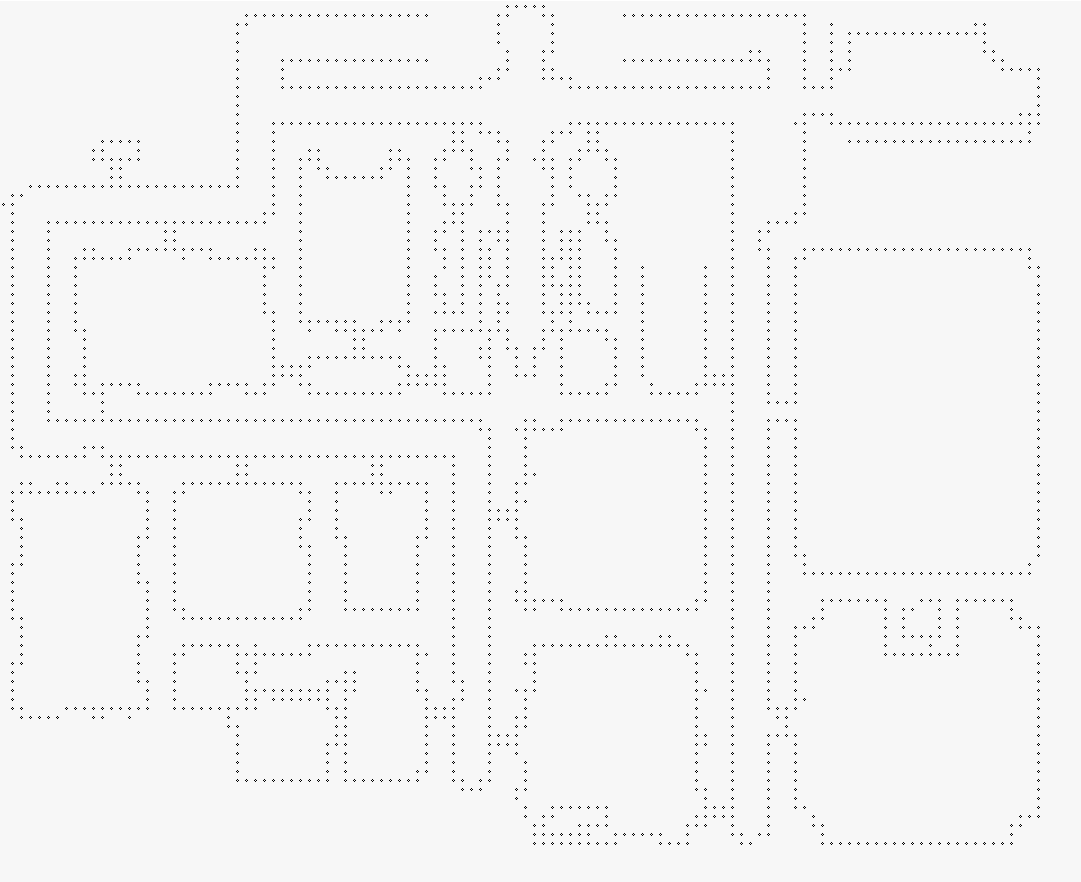
\includegraphics[width=6cm, height=3cm]{SpatialKnowledge/floor0}}
   %  \hspace{1pt}
    \subfloat[Ground Floor]{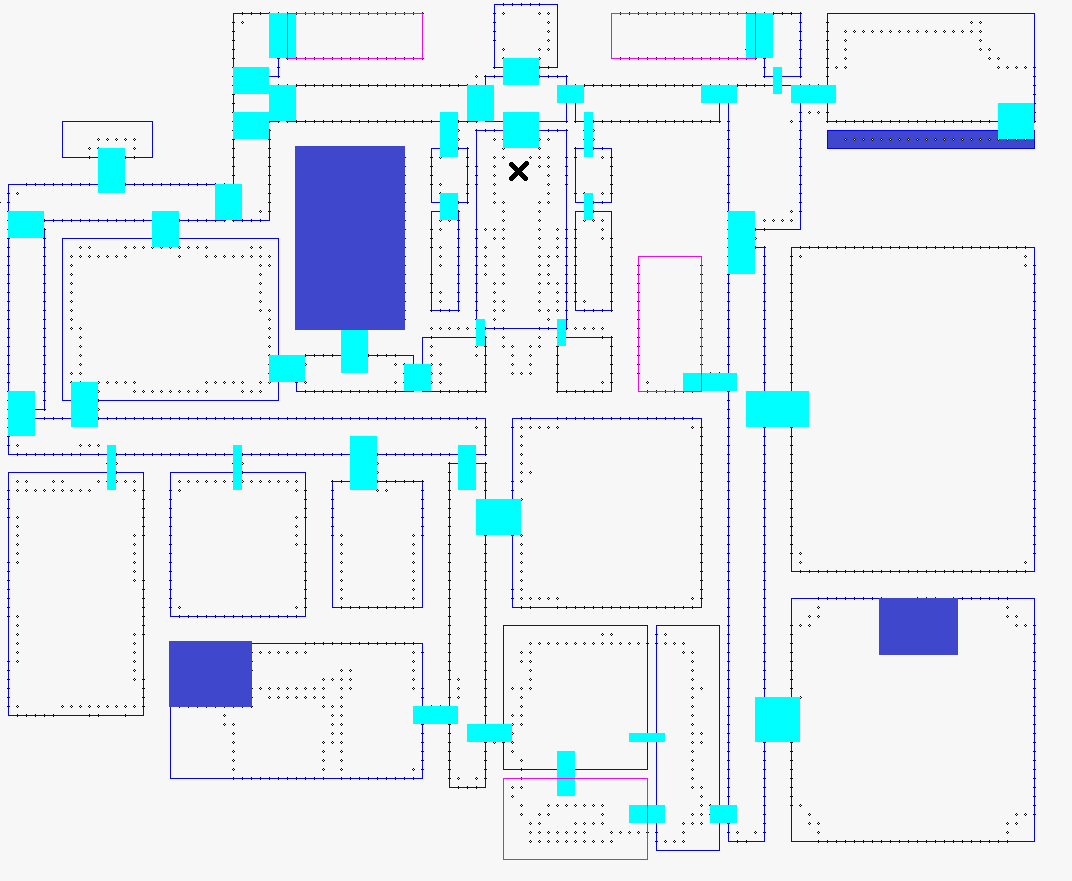
\includegraphics[scale=0.28]{SpatialKnowledge/floor0WithRooms}}
   \\
  %  \subfloat[First Floor]{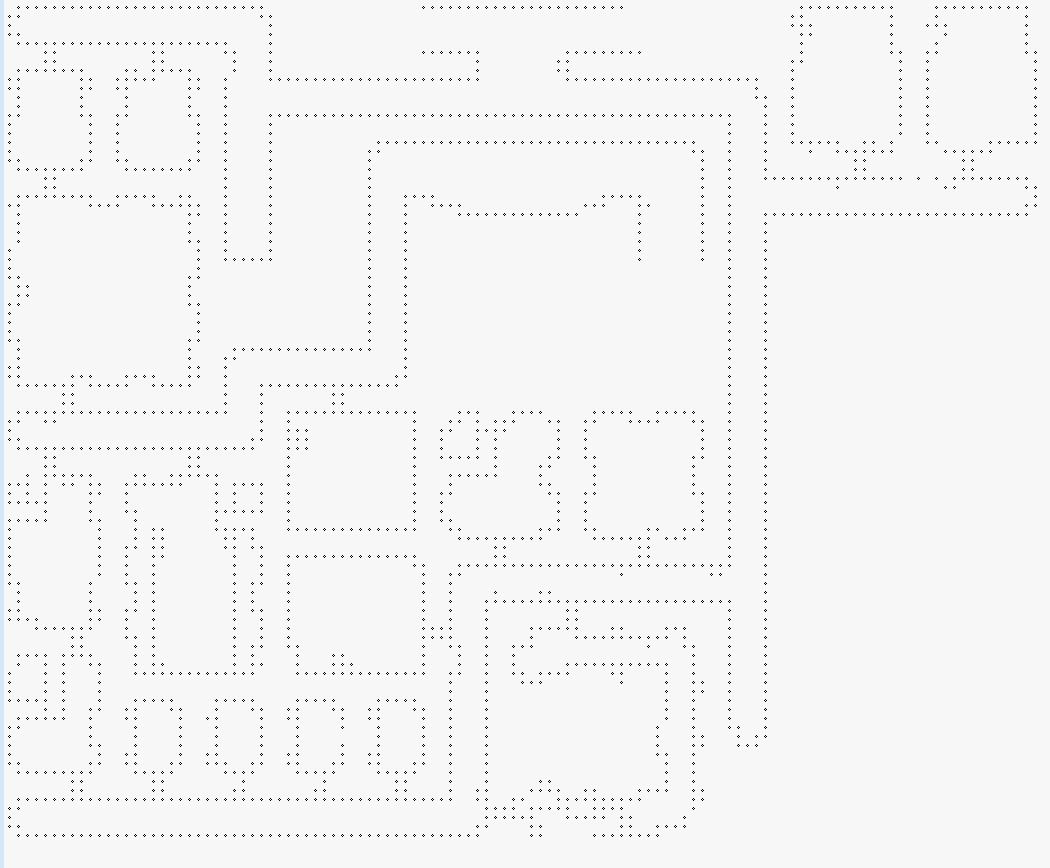
\includegraphics[width=6cm, height=3cm]{SpatialKnowledge/floor1}}
  % \hspace{1pt}
    \subfloat[First Floor]{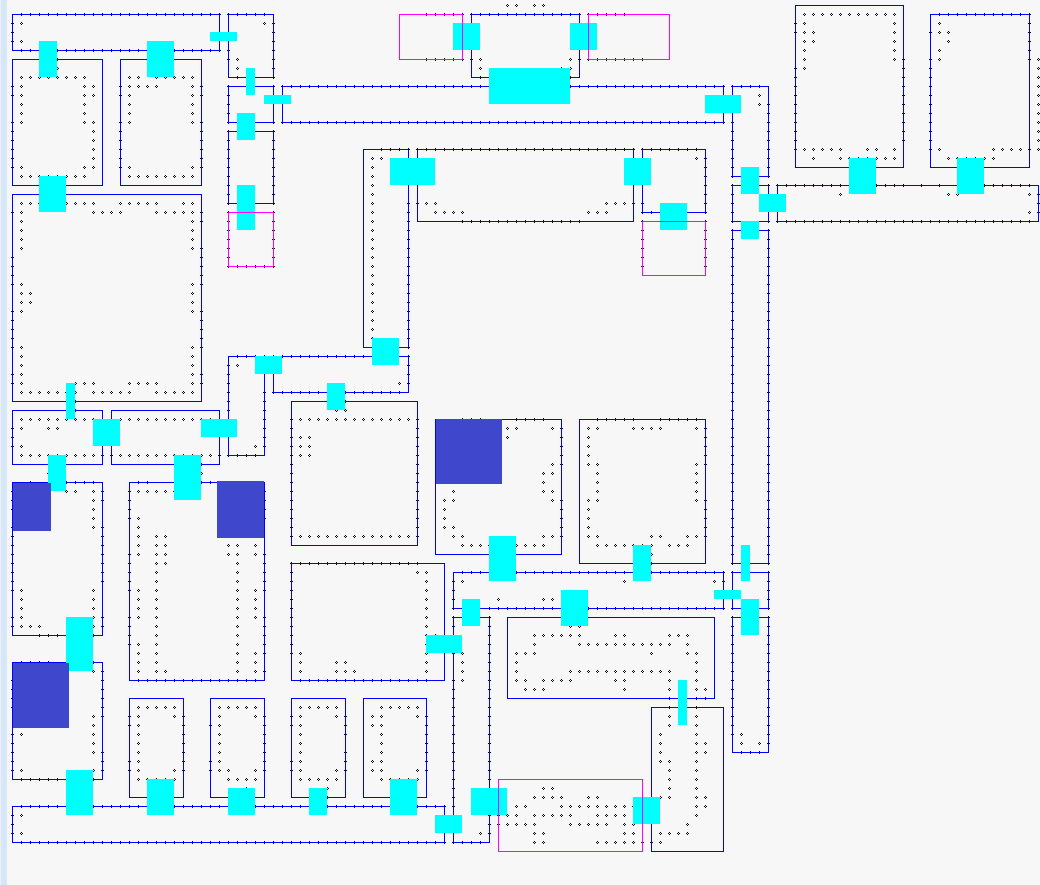
\includegraphics[scale=0.28]{SpatialKnowledge/floor1WithRooms}}
  \\
  % \subfloat[Second Floor]{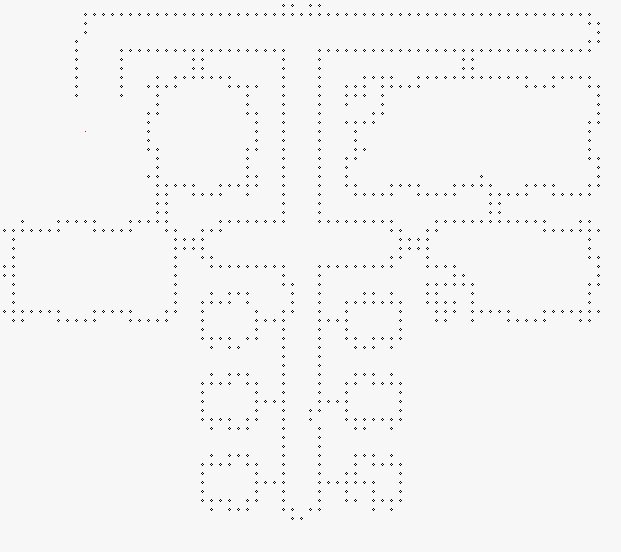
\includegraphics[width=6cm, height=3cm]{SpatialKnowledge/floor2}}
  % \hspace{1pt}
  \subfloat[Second Floor]{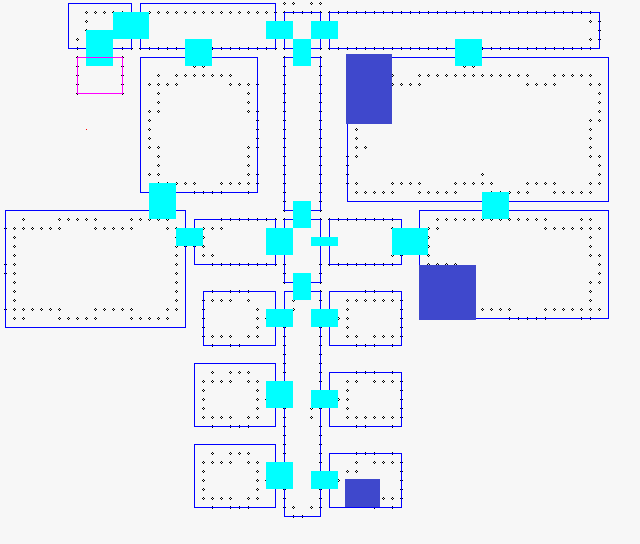
\includegraphics[scale=0.28]{SpatialKnowledge/floor2WithRooms}}
  \caption[Floor Plans of the three floors]{Floor Plans of the three floors. The X indicates the starting point. The blue color indicates the prisoner locations. It is a modified version of an existing Minecraft map~\cite{RoyalPalaceMap}}
  \label{fig:FloorPlans}
\end{figure}



The next phase, which we call \emph{knowledge testing phase}, starts when the eleventh prisoner has been freed. During this phase, the cognitive map formed by the player is tested through a series of three tasks, which involve operating switches that were hidden during the exploration phase. By not revealing the nature of the second phase to the player at the beginning of the game and also by hiding the location of the knowledge testing tasks, we ensure that the player does not make a special effort in remembering locations which could artificially alter the cognitive map formed.

When the eleventh prisoner is freed and the exploration phase ends, the player is given instructions to proceed to the gallery room (shown in Fig.~\ref{fig:MinecraftEscapePaintingRoom}). This room would have been examined by the player during exploration. It is the only room in the palace whose walls are covered with paintings and this makes it reasonably likely that the player will remember this location because of its \emph{perceptual salience}~\cite{Davis01122009}.
% Majority of the players remembering this location indicates that perceptua is indeed a key factor in remembering locations.


\begin{figure}[!tb]
    \begin{center}
        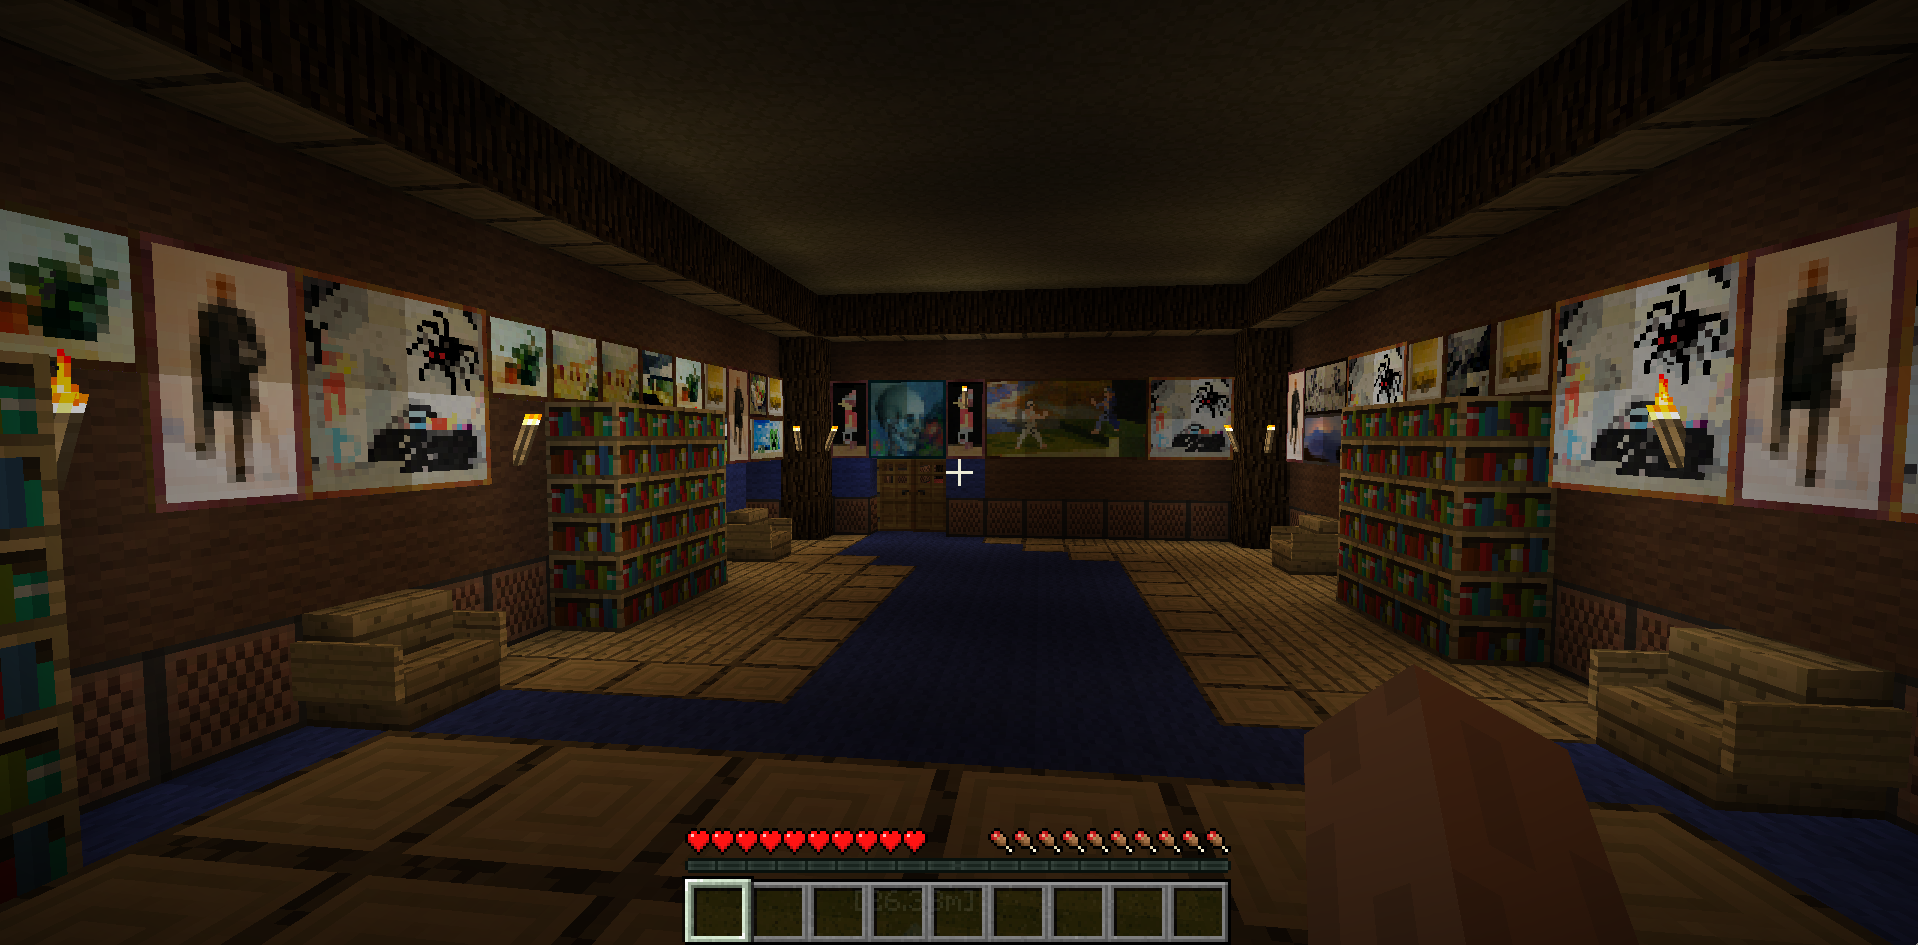
\includegraphics[width=\textwidth]{SpatialKnowledge/PictureGallery}
    \end{center}
    \caption{Picture Gallery}
    \label{fig:MinecraftEscapePaintingRoom}
\end{figure}
%mhl - perhaps give a screen shot of the gallery?

Once the player locates and presses the switch that is revealed in this room, the player is given instructions to move to the second floor library. There are two important factors for choosing this particular location. Firstly, the library has four entrances and is very likely that the player would have entered this room multiple times during the exploration phase. Secondly, being on the second floor, there are multiple paths to this location from the gallery.
% Preference for a particular route among players would help understand more about his/ her cognitive map.

Once this location is found, the player is given the final instruction to proceed to their starting location to find the final switch that will open the main gate to the palace. Again, there are multiple routes to this location some of which are significantly shorter than others. Also, being a starting location and in a somewhat central location, it is likely that it has been frequently visited and should have some \emph{cognitive salience}~\cite{Davis01122009}. We built the experiment inside the popular game Minecraft~\cite{Minecraft} in order to reduce the development effort and to allow for flexibility in environment creation.


\subsection{The Minecraft gaming environment}
\label{sec:the_minecraft_gaming_environment}

Minecraft~\cite{Minecraft} is a Java based multi-platform sandbox construction game. The game involves players creating and destroying various types of blocks in a first-person three-dimensional environment. In the original game, the player controls an avatar that can destroy or create blocks, forming buildings, structures, artwork and even entire cities on multi-player servers or single player worlds across multiple game modes. Players can break any block and build any block, provided he/she has the resources. Figure~\ref{fig:MinecraftEscapePaintingRoom} gives a better idea of the look and feel of the game.


In the development of the game described in the previous section, we use an existing plug-in~\cite{BukkitPermissions} that constrains players so that they can only move around in the environment and interact with doors and switches, that is, elements that are essential for the experiment. A second modification is used~\cite{MyStatisticsPlugin} to keep a log of the movements and actions of the players and store them in a MySql server for analysis. The player locations at different times, the time at which each prison was opened and the time taken to complete each task in the testing phase are all recorded for this purpose.

Using Minecraft provided several advantages; being a popular game with standard controls and a first person view, immersiveness and interestingness are much easier to achieve. Another useful consequence of the popularity of minecraft is the large community of developers and the number of Java based plugins that are available for modifying the default Minecraft environment. This made it easier to develop the game and make the necessary modifications to make the experiment as required. However, the biggest advantage of using Minecraft is the ubiquity it offers with over 35 million copies sold. If hosted on a publicly accessible server, it would be theoretically not be difficult to get several hundred, if not thousand participants. Efforts that have been made to do this are presented in Section~\ref{sec:scaling_the_game}. In the present chapter, we present the initial results of the game being played by participants on a local server.


% section benefits_of_the_proposed_approach (end)
\subsection{Participants} % (fold)
\label{sec:participants}

Fifty young adults (14 women, 36 men, age range: 18-30 years) were recruited with fliers posted on the Nanyang Technological University Campus. Participants were compensated \$ 5 for their participation in the game. It was played by all participants on the same computer in a lab with minimal distractions.

Participants were given five minutes to familiarize themselves with the controls of the first person game, which involved using the keyboard direction keys for movement and the mouse for altering the move and view direction. A mouse click would allow the player to interact with the environment by either opening doors or freeing prisons. The players were given 45 minutes to complete the game. Of the 50 participants, the data from only 44 participants were used, the remaining six experienced motion sickness from the movement in the first person gaming environment and had to quit playing before the game could be completed. Next, we explain the way in which the data was analyzed.

% section participants (end)
\section{Analysis} % (fold)  % To find a better name
\label{sec:methodologies}

In this section we present the methods that were used to analyze the data obtained from the game. Figure~\ref{fig:UnscaledMap} shows the room layout show in Figure~\ref{fig:FloorPlans} as an undirected a graph. A directed \emph{movement graph} is calculated for each player, with the edges of the graph indicating the direction and time of movement from one node to the next. The analysis presented in the following sections is performed using these graphs.


\begin{sidewaysfigure*}[!htbp]
\centering
\includegraphics[width=\textwidth]{SpatialKnowledge/unscaledRoomLayout.pdf}
\caption[Graphical representation of floor plan]{This figure shows a graphical representation of the room layout in Figure~\ref{fig:FloorPlans}}
\label{fig:UnscaledMap}
\end{sidewaysfigure*}



\subsection{Types of exploring agents}
\label{sec:types_of_data}

As mentioned in the introduction, the motivation of our analysis is to determine how memory influences exploration efficiency and an individual's ability to navigate within an environment. In order to do this, we use an approach similar to the ideal navigator model of  Stankiewicz et al~\cite{stankiewicz2006lost}. We compare the movement of the players to different kinds of simple exploring agents inhabiting the same environment as the player. By comparing the performance of these simple agents to the actual performance of the player, we determine the ways in which a player is different from or similar to each of these agents.

We compare the \emph{movement graph} of the players to three kinds of exploring agents: Markov agents, unbiased random walkers and agents with perfect $m$-step memory. Just like the actual players, these agents have no prior knowledge and explore the undirected graph shown in Figure~\ref{fig:UnscaledMap}. Our analysis is done based on four sets of directed movement graphs :
\begin{itemize}
    \item \emph{Actual Players}: This is the set of 44 player movement graphs i.e. the movement graphs introduced at the beginning of this Section.

    \item \emph{Unbiased Random Walker}:  The next node to which this agent moves is chosen randomly with equal probability. Each iteration of the random walk is performed until the walker covers $100\%$ of the environment. A collection of random walks is obtained until the variance in the radius of gyration of generated movement graphs stabilizes. The radius of gyration is the standard deviation of a walker's position to the center of mass of movement~\cite{cheng:footprints}. It gives a measure of the locality of the graph.

    \item \emph{Agent with perfect $m$-step Memory}: This is a biased random walker with an $m$-step memory. It moves exactly like the random walker except that it avoids moving back to any of the $m$ rooms it visited previously. If there is no unvisited room, the agent checks its $m$-step memory for an unexplored junction. If such a junction exists, it goes back to that point and continues exploring in an unvisited direction. If such a junction does not exist the agent simply choses,  at random,  a neighbouring location to the current node with equal probability. Depending on the calculation being performed, the path is generated for a specific number of hops or until a specific coverage is achieved. The coverage is simply calculated as:
    \begin{equation}
        \mbox{coverage} = \frac{\mbox{number of rooms visited}}{\mbox{total number of rooms}} \times 100
        \label{eq:CoverageEquation}
    \end{equation}
     $30,000$ such movement graphs are generated for each value of $m$ for each experiment. This was empirically found out to be a good enough value to ensure minimal variation in the radius of gyration.

    \item \emph{$m^{th}$ order Markov Agents}: These agents mimic the movement of the average of the ensemble of players assuming they had only an $m$ step memory. The action of an $m^{th}$ order Markov agent at a particular point in the path is a function of the actions of the actual players who had taken the same $m$ steps. This is explained in more detail in Section~\ref{sec:Markov_data_analysis}. The calculations are performed for m from 1 to 13. As with the agent with perfect memory, the movement graphs are generated either for a specific number of hops or until a specific amount of coverage is achieved. Also, as before, $30,000$ movement graphs are generated for each value of $m$.
\end{itemize}

Simulations of movement were used to generate movement graphs for each of these types of agents and the results of this analysis are presented in Section~\ref{sec:analysis_of_experiment_results}. Before this, the next section explains the working of the Markov agents in more detail.

\subsection{Markov Agents}
\label{sec:Markov_data_analysis}


In this section we present how the movement of the Markov agents are calculated. The chief motivation of this Markovian analysis was to investigate the role that memory plays in the exploration of the environment.

We take an $m^{th}$ order Markov model to represent an $m$-step memory of the explorer, where steps constitute node visits on the undirected graph (Figure~\ref{fig:UnscaledMap}). One way to speculate on the size of the memory used by a human during exploration is to predict a path of length $n$ from some Markov data of order $m < n$.  We hypothesize that \emph{if the movement of the actual players can be predicted using an $m^{th}$ order Markov agent, this implies that humans use a working memory of size $m$ steps during exploration.}

In a general $m^{th}$ order Markov process, the basic idea is that the action at any point of time depends only on the previous $m$ actions. By stating that the process of exploration is an $m^{th}$ order Markov process, we assume that the next node that is visited by a player is only dependent on the previous $m$ steps. This is different from an agent with $m$-step memory that tries to avoid the previous $m$ nodes. Since the next step is dependent on the actions of players who have visited that same subsequence of $m$ nodes, the Markov model theoretically encapsulates other factors like layout, visibility and so forth and thus unlike the former, has \emph{imperfect recollection}.


\begin{figure}[!t]
\centering
        \subfloat[The Situation]{\label{fig:situation}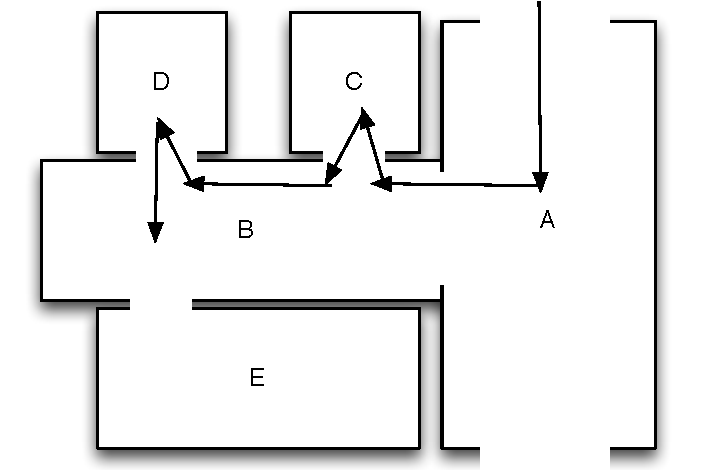
\includegraphics[width= 0.48\textwidth]{SpatialKnowledge/situation}}
    \hspace{1pt}
        \subfloat[Player 1]{\label{fig:player1}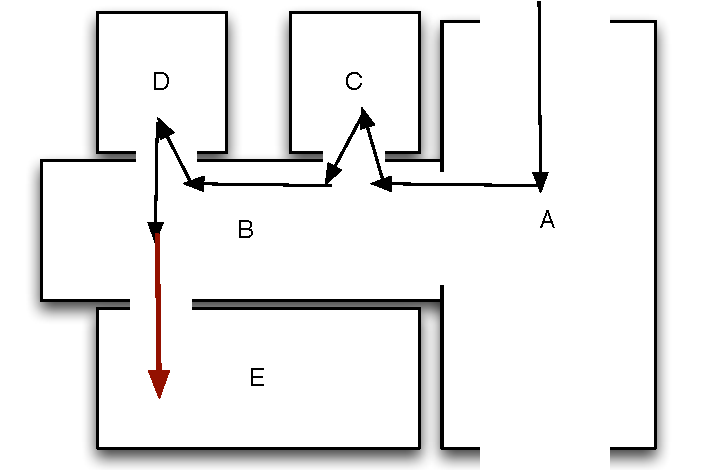
\includegraphics[width= 0.48\textwidth]{SpatialKnowledge/player1}}
    \\
        \subfloat[Player 2]{\label{fig:player2}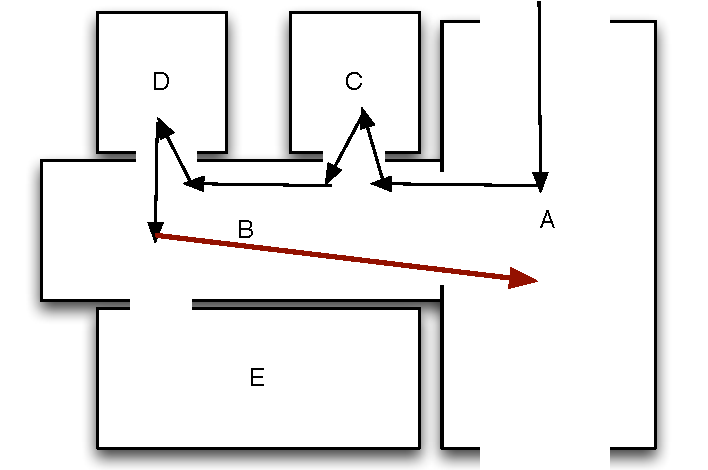
\includegraphics[width= 0.48\textwidth]{SpatialKnowledge/player2}}
    \hspace{1pt}
        \subfloat[Player 3]{\label{fig:player3}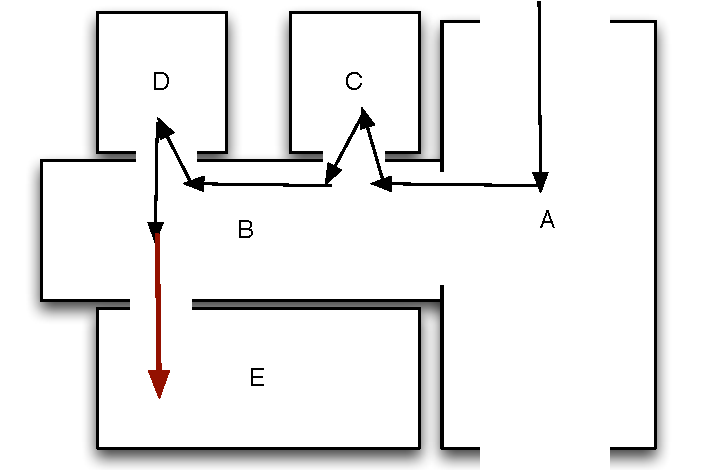
\includegraphics[width= 0.48\textwidth]{SpatialKnowledge/player3}}
    \\
        \subfloat[Agent with 6-step memory]{\label{fig:agent}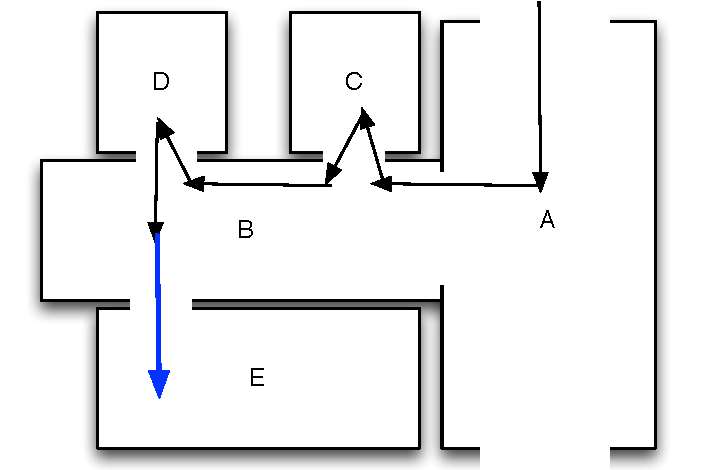
\includegraphics[width= 0.48\textwidth]{SpatialKnowledge/agentWithMemory}}
    \hspace{1pt}
        \subfloat[$6^{th}$ order Markov Agent]{\label{fig:markov}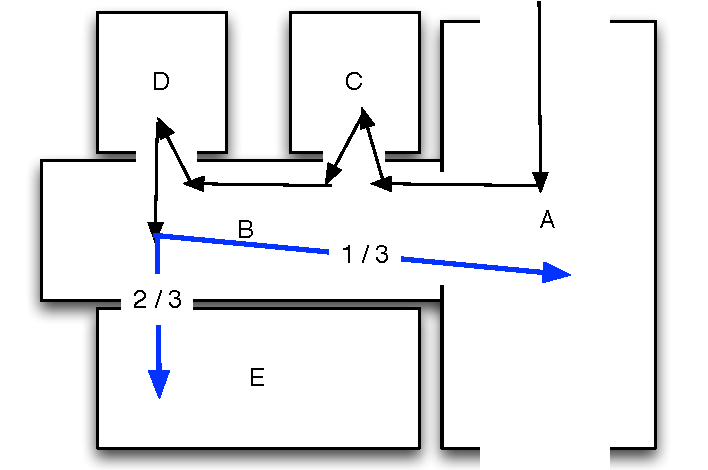
\includegraphics[width= 0.48\textwidth]{SpatialKnowledge/markovAgent}}
    \caption[Markov Data Explanation]{Given the situation in (a), the agent with 6-step memory would move next to room E since it has the list {B,D,B,C,B,A} as the 6 rooms visited immediately previously. However, the action of the $6^{th}$ order Markov agent in this situation is dependent on the actions of the players ((b),(c) \& (d)) who happened to be in the same situation. Since one out of the three players who were in the given situation next moved to room A, there is a $1/3$ chance that the Markov agent will visit room A next.}
    \label{fig:markovExample}
\end{figure}


Figure~\ref{fig:markovExample} explains the idea of a Markov agent by contrasting it's behavior with that of an agent with simple m-step memory. In the example layout shown in figure--- with the rooms C, D and E connected to corridors A and B--- we consider the situation where the exploring agent has moved from A to B to C to B to D and back to B. Assuming a 6-step memory, the simple memory agent would definitely visit room E since all other rooms have been visited in the last 6 steps. However, the Markov agent's action in this situation depends on the actions of the actual players in this situation. Since two out of the three players visited room E and one out of the three players visited room A, the next step of the Markov agent can either be room E or A with $2/3$ and $1/3$ probability respectively. The following section explains in more detail how the Markov agent movement graphs are calculated.
% Interestingly we found significant performance improvements when we reach $m$ of 6 to 8.

% To understand if an $m^{th}$ order Markov model is sufficient for describing exploration efficiency we measure the exploration performance in terms of minimum hops needed and maximum coverage obtained. This is done for different values of $m$ and then compared with the exploration of the unbiased random walker and the agent with perfect $m$-step memory.

\subsubsection{Calculation of Markov data} % (fold)
\label{sec:calculation_of_Markov_data}

\begin{table*}[!bp]
\caption{Summary of symbols and their meaning.}
\label{tab:Symbol_Table}
\begin{tabular}{lcc}\hline

Symbol & Meaning   \\ \hline
$Pr (A|B)$ & Probability of occurrence of event A given event B \\
$X_n$ & Random variable indicating the location in the $n^{th}$ step \\
$p^{(n)}_{ij}$ & Probability of going from state $i$ to state $j$ in $n$ steps \\
$R$ & Set of all nodes \\
$r$ & A particular node \\
$N_r$ & Set of neighbors of node $r$ \\
$P^{(n,D)}$ & List of all paths of length $n$ taken by individuals in dataset $D$\\
$Q^{(n)}$ & Random variable representing a path of length $n$\\
$q^{(n)}$ & A particular path of length $n$\\
$\phi(a,L)$ & The number of occurrences of element $a$ in list $L$\\
$x^{(q)}_{i}$ & The $i^{th}$ location in a particular path $q$\\

\hline
\end{tabular}
\end{table*}

This section explains how the aforementioned Markov calculations are done. These calculations are performed on the \emph{actual player} dataset $D$ derived from the game (Section~\ref{sec:types_of_data}). To recap, a directed movement graph is stored for each player. Each node of the directed movement graph corresponds to a node in Figure~\ref{fig:UnscaledMap} and each edge indicates the movement of the player from one node to the next. Each edge also stores the time point of traversal. The symbols used in this section and their meaning are summarized in Table~\ref{tab:Symbol_Table}.


The $m^{th}$ order Markov probability of visiting a node $b$ from a node $a$ is defined as the probability that the $m^{th}$ node after visiting node $a$ is node $b$. Mathematically, it can be stated as:
\begin{equation}
    p^{m}_{ab} = Pr(X_{m}=b|X_{0}=a)
\end{equation}

It is assumed that it is a time homogeneous process, that is,
\begin{equation}
    p^{m}_{ab} = Pr(X_{k+m}=b|X_{k}=a) \ where\  k \geq 0
\end{equation}



To calculate the $m^{th}$ order Markov data using dataset $D$, we calculate the following:
\begin{enumerate}
    \item First, for each path of length $m$, \emph{the number of times that path is observed} in dataset $D$ is counted.

    From this, the following equation can be used to derive $p^{m}_{ab}$:
    \begin{equation}
        p^{m}_{ab} = \frac{\left\vert{P^{(m,D)}_{ab}}\right\vert}{\sum\limits_{x\in R}\left\vert{P^{(m,D)}_{ax}}\right\vert}
        \label{eq:HeatMapEquation}
    \end{equation}

    \item For each path of length $m$, \emph{the likelihood that a particular path} is the result of $m$ steps being taken is simply the ratio of the number of occurrences of the particular path of length $m$ to the total number of paths of length $m$ in the database $D$; mathematically:
    \begin{equation}
        Pr(Q^{(m)}=q^{(m)}) = \frac{\phi(q^{(m)},P^{(m,D)})}{\left\vert{P^{(m,D)}}\right\vert}
        \label{eq:TableEquation}
    \end{equation}


    \item Using these, we can calculate the probability of each destination given a particular path of length $m$ by using Bayes Theorem.


\end{enumerate}

For $m^{th}$-order Markov agent, given a particular path of length $m$, it is possible to generate the $(m+1)^{th}$ step using the previous $m$ steps, that is, the $1^{st}$ to $m^{th}$ step. This is done using the destination probabilities calculated in step 3. Following this, the $(m+2)^{th}$ step can be predicted by doing the same calculation using the preceding $m$ steps from $2$ to $m+1$. This process can be continued to generate a directed movement graph of $n$ edges using just the $m^{th}$ order Markov data. As mentioned previously, calculations are done using $30,000$ paths generated like this. A question that might arise for the discerning reader at this point is whether the dataset is sufficiently large to do such Markov calculations reliably for large values of $m$. We present further analysis on the validity of this calculation in Appendix~\ref{sec:validity_check_for_markov_analysis}. Next, we look at the results of our analysis.

% section methodologies (end)

\section{Results} % (fold)
\label{sec:analysis_of_experiment_results}

% VVT: WRITE AN ACTUAL INTRODUCTION TO THIS SECTION!!
% In the previous section we introduced the basic techniques that we used for analyzing the data obtained from the games. In this section we present our findings from using these techniques on the data.

% \begin{sidewaysfigure*}[!htbp]
% \centering
% \includegraphics[width=\textwidth]{SpatialKnowledge/unscaledRoomLayout.pdf}
% \caption{This figure shows a graphical representation of the room layout in Figure~\ref{fig:FloorPlans}}
% \label{fig:UnscaledMap}
% \end{sidewaysfigure*}

From the game, the complete movement traces of 50 players were obtained. This data was analysed by comparing against agents of different types to determine patterns and gain a better understanding of the movements of the players. This section presents the results of four kinds of analysis that was performed. First, we present the results of a simple check of the frequency of visits to each room. Following this, we compare the efficiency of movement of the players against the different agents. Finally, we present some empirical observations from the movement graphs of the actual players.


\subsection{Room visit frequencies}


In our first experiment, we calculate the frequency of visits for each room per player and compare this against the unbiased random walker. This is a simple test to determine if the players have a pattern or strategy in their exploration that is different from a random walk. If there is a significant difference in the number of times a particular floor or area of the building is visited by a player then this will probably be revealed by this comparison against an unbiased random walker.

For each room $r$ we calculate the normalized number of visits $\alpha$. For any room $r$, let $f_p(r)$ be the total number of times room $r$ is visited by the the player $p$ and let $f_{rw}(r)$ be the number of times the average random walker visited the same room. We define the normalized number of visits $\alpha$ as:
\begin{equation}
	\alpha_x(r) = \frac{f_x(r)}{\sum_{a \in R} f_x(a)}
	\label{eq:alpha_equation}
\end{equation}
This is calculated for both the player and the random walker. Using this the visit ratio, $y_{p}(r)$, of the actual player is calculated for each room as:
\begin{equation}
y_{p}(r) = \frac{\alpha_p(r)}{\alpha_{rw}(r)}
\label{eq:y_equation}
\end{equation}
A random walker's frequency of visits to a particular node is purely a function of the topography of an environment i.e. the nodes and their connectivity. Thus, unlike $\alpha_p(r)$, $y_p(r)$ would not contain the effects of the degree of a node. This means that if a room $r_1$ has lower value of lower $y_p(r)$ than $r_2$, this is not because of the room having lesser connectivity. The average $y(r)$ over the ensemble of player data was then calculated. This is illustrated in Figure~\ref{fig:scaledMap}. This figure shows the value of $y(r)$ of each room as a scaled version of Figure~\ref{fig:UnscaledMap}. The red color indicates those rooms that have $5\%$ more visits than a random walker and the green color indicates those that have $5\%$ less visits than a random walker; the node is colored white otherwise. The diameter of each node in this graph is scaled to $y_r \times \mbox {unscaled diameter}$.

\begin{sidewaysfigure*}[!htbp]
\centering
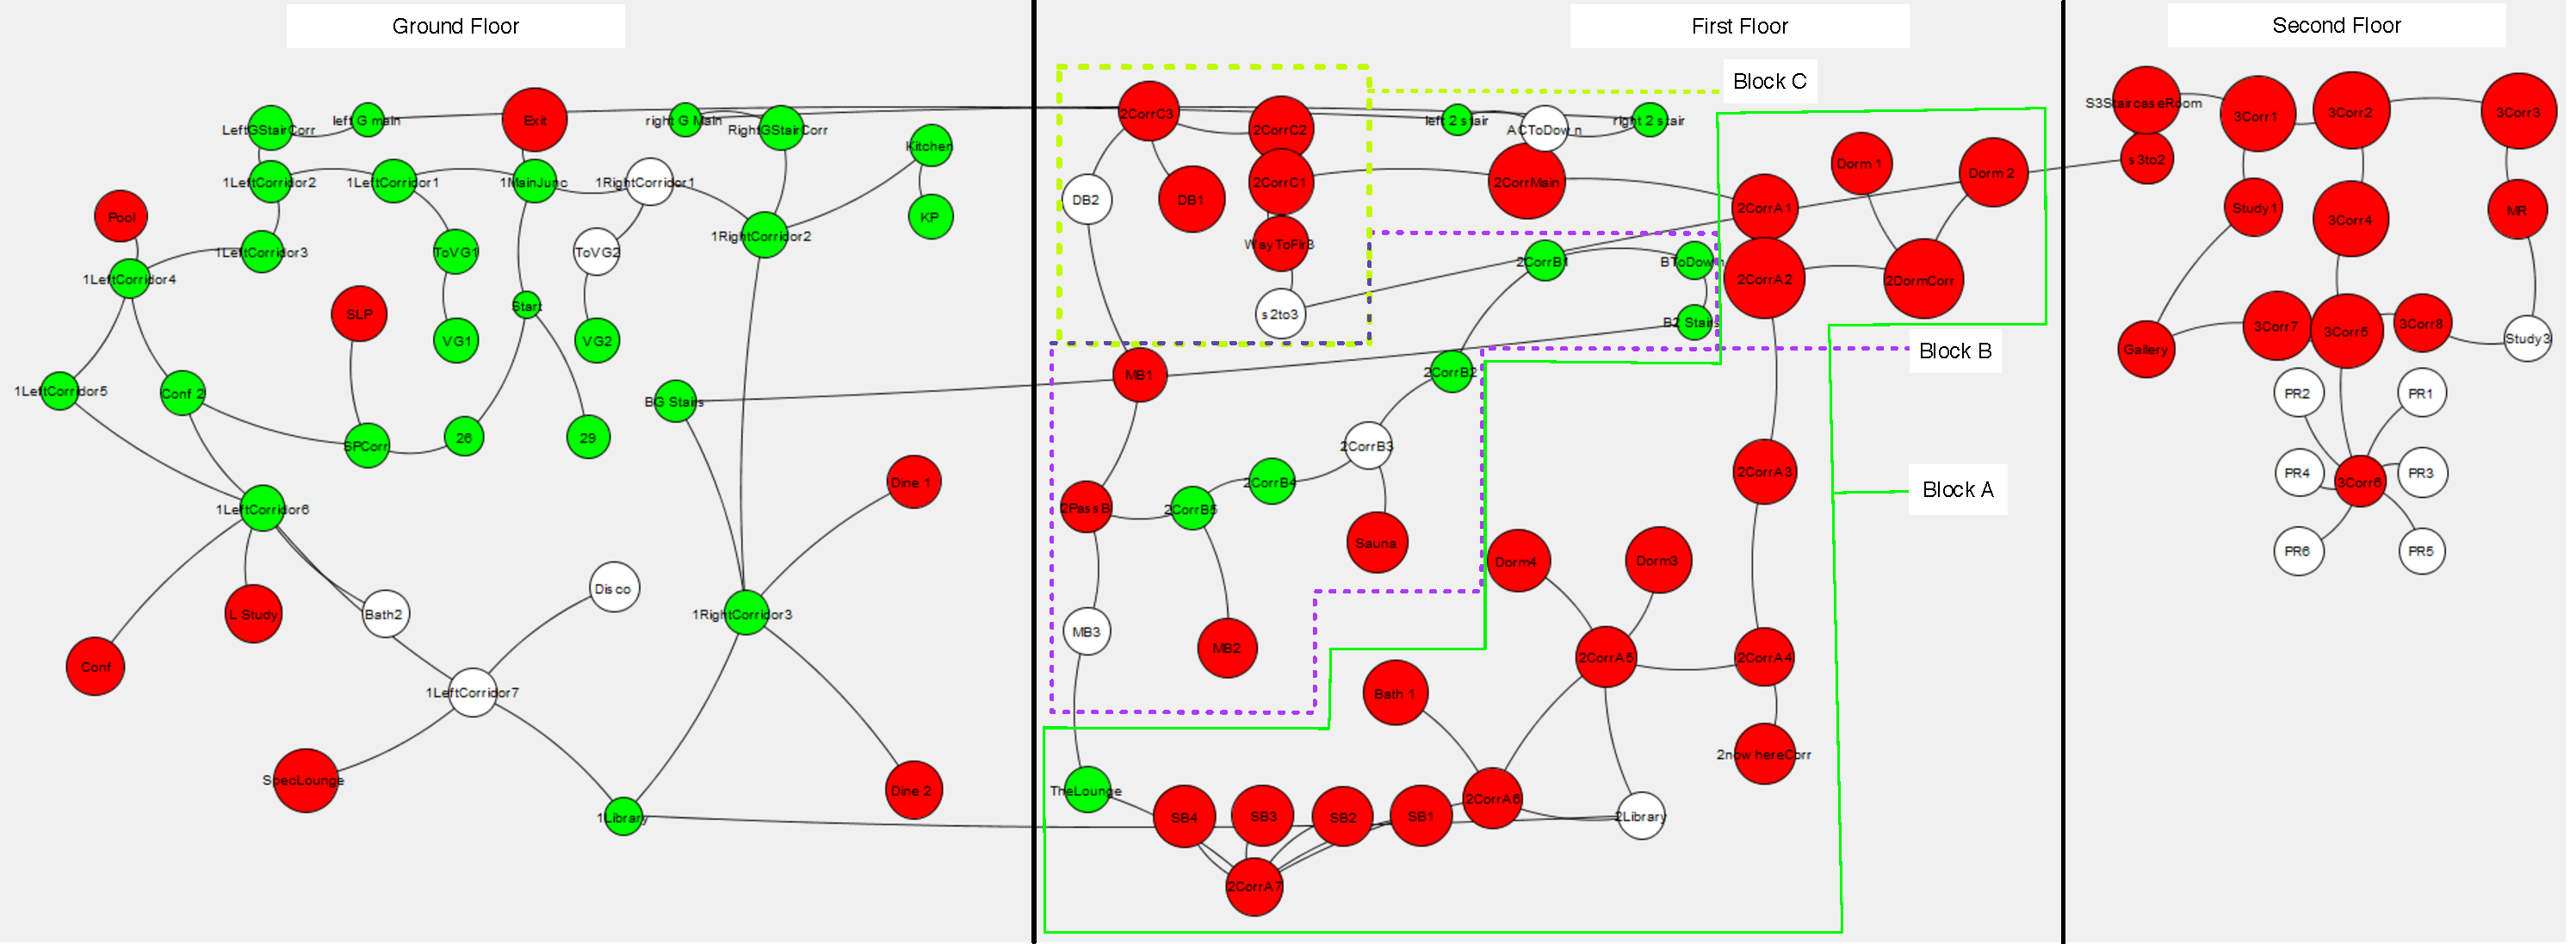
\includegraphics[width=\textwidth]{SpatialKnowledge/scaledGraph.pdf}
\caption[Visualization of room visit frequencies]{Figure~\ref{fig:UnscaledMap} scaled by normalized number of visits as described in Equation~\ref{eq:y_equation}. Red color indicates a $y$ value of greater than $1.05$ and the green color indicates a value of less than $0.95$ . The diameter of each node in this graph is scaled to $y_r \times (unscaled\ diameter)$.}
\label{fig:scaledMap}
\end{sidewaysfigure*}

Therefore, a white color indicates that the normalized number of visits in both the \emph{random walker} dataset and in the \emph{actual player} dataset are within 5\% of each other. A value greater than 1 indicates that players visited the room more than the random walker and a smaller value indicates the opposite. It is hard to discern any pattern in Figure~\ref{fig:scaledMap}, other than the fact that there is a marked difference in the visits by the players and visits by the random walker. However, it can be seen that the average number of visits on the second floor was higher than the number of visits on the first floor which was more than the number of visits on the ground floor.

Despite a random walker not differentiating between staircases and other links, a random walker might have more visits to one floor than another purely because there are fewer inter floor connections than other links. For example, floor 3 has only one staircase that leads the random walker out of the third floor. To confirm that the inter floor differences for the actual player is not because of this, we normalize Equation~\ref{eq:alpha_equation} to the number of visits on the floor rather than the total number of visits. On doing this, if the graph is different form Figure~\ref{fig:scaledMap}, it would seem that unlike a random walker, a player differentiates between a simple link between rooms or corridors and a staircase which is a link between floors. Figure~\ref{fig:scaledGraphByFloor} which is the floor normalized version of Figure~\ref{fig:scaledMap} does clearly show this.

% \begin{sidewaysfigure*}[!htbp]
% \centering
% \includegraphics[width=\textwidth]{unscaledRoomLayout.pdf}
% \caption{This figure shows a graphical representation of the room layout in Figure~\ref{fig:FloorPlans}}
% \label{fig:UnscaledMap}
% \end{sidewaysfigure*}

\begin{sidewaysfigure*}[!htbp]
\centering
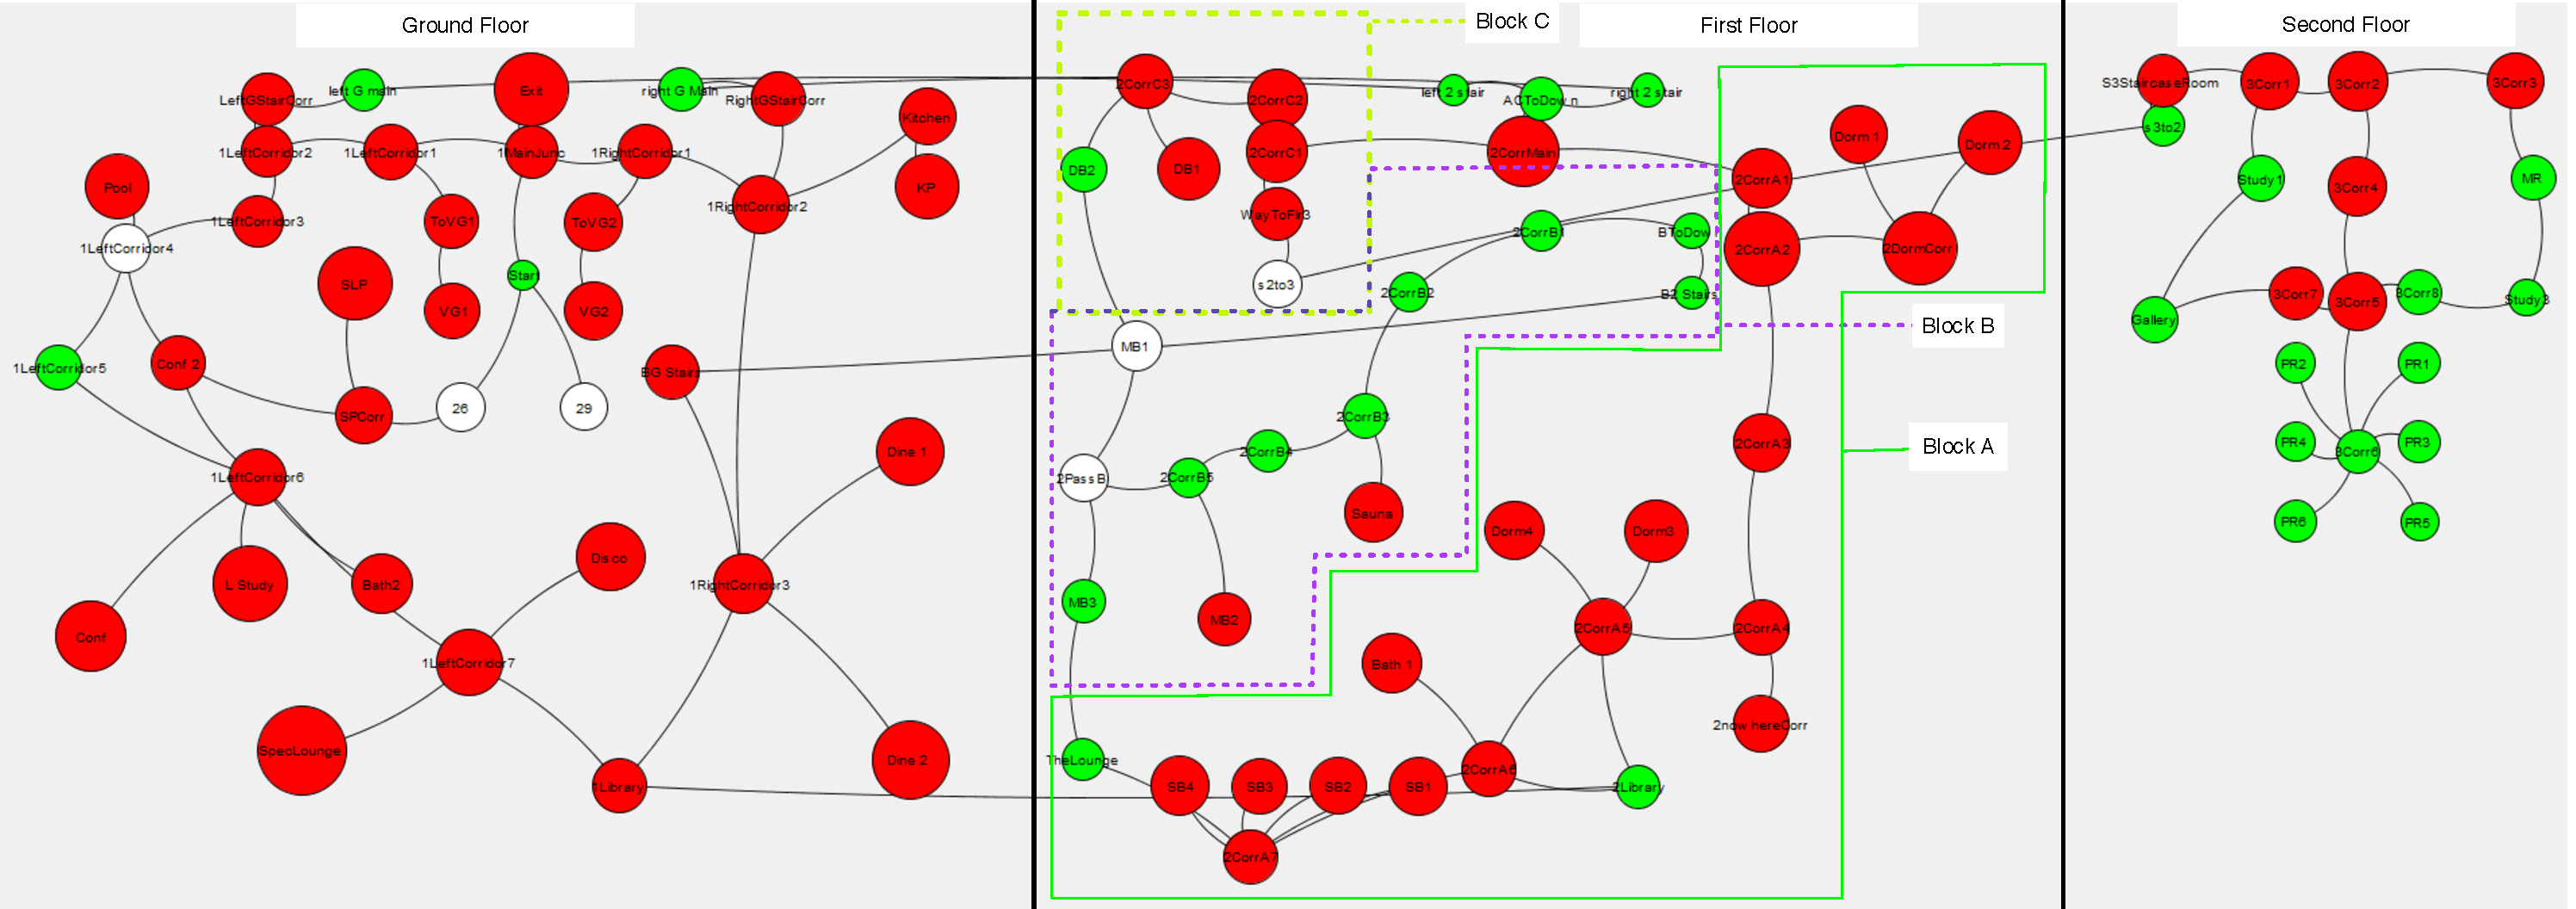
\includegraphics[width=\textwidth]{SpatialKnowledge/scaledGraphPerFloor.pdf}
\caption[Room visit frequencies normalized to floor]{Figure~\ref{fig:scaledMap} normalized to floor instead of the total number of visits. The fact that this graph is different from Figure~\ref{fig:scaledMap} indicates that, unlike a random walker, a player differentiates between a simple link between rooms or corridors and a staircase which links two floors.}
\label{fig:scaledGraphByFloor}
\end{sidewaysfigure*}

Figure~\ref{fig:scaledMap} and~\ref{fig:scaledGraphByFloor} provide a possible validation of a variation of the floor first strategy~\cite{HolscherBMS06} used for exploration. The strategy in the original paper was for wayfinding with a particular goal, but here it seems to be being used for exploration (which is wayfinding without a definite goal). The players seem to consider each floor as a separate entity and are generally reluctant to take the staircase. This might also be because the process of separating each floor helps in bringing some organization and structure to the confusing room layout and the process of exploration (that is, completely explore one level before the next).

There is a chance that this aversion to taking staircases is a consequence of the structure of the game environment or the controls in the game. This would happen if the staircases were difficult to find or climbing staircases required different controls from moving through doors or walking through corridors. However, this is not the case in the designed game. The player just has to press the forward button to move in the environment regardless of whether it is a staircase or a corridor or a room. Also, the staircases are clearly visible from the neighboring nodes with sign boards further confirming their location.
%  FIGURE : Do we need a figure of a staircase here?

The hypothesis of the existence of this floor first strategy is further strengthened by the low visit frequencies to Block B on the second floor~\ref{fig:scaledGraphByFloor}. There are four staircases that take a player from floor 1 to floor 2: two of these lead to Block A, one to Block C and one to Block B. Block A and C are directly connected by a corridor whereas the only paths to Block B from the same floor are through rooms DB2 and The Lounge in Block A and C respectively. This means that, unlike Block A and C, Block B is not accessible via any direct corridor from the same floor. Since people show a clear inclination to exploring through corridors as shown in Section~\ref{sec:empiricalanalysis} of this chapter, the only obvious way to access Block B is by going down a floor. The fact that Block B has fewer visits seems to suggest that people resist going down a floor. Thus further strengthening the hypothesis of a floor first strategy in exploration.

% section types_of_data (end)

\subsection{Expected coverage given number of hops} % (fold)
\label{sec:calculation_4_expected_coverage_given_number_of_hops}

The average coverage after a given number of hops gives an estimate of the efficiency and effectiveness of exploration. On average each player took $252.6 \pm 7.5$ hops during their exploration phase. The coverage achieved by the other types of agents after 253 hops was calculated by generating the required set of movement graphs as explained in Section~\ref{sec:types_of_data}. Figure~\ref{fig:coverage} shows the results of this calculation.


\begin{figure*}[tb]
    \begin{center}
        \includegraphics[width=\textwidth]{SpatialKnowledge/coverage-253.PNG}
    \end{center}
    \caption[Expected coverage after 253 hops]{This figure shows a standard error plot of the average coverage after 253 hops as a function of memory size. The low values of standard error on the agent paths are because these calculations are calculated over several thousand paths that are required for the radius of gyration to stabilize. A value of 253 hops was taken because this was the average number of hops taken by a player.}
    \label{fig:coverage}
\end{figure*}


The figure seems to indicate that even a second order Markov agent, that is, one whose next position is only dependent on its current and previous position, performs much better than an unbiased random walker. It also seems to indicate that after 253 hops the performance of the actual players is much better than both the Markov agent and an agent with an $m$-step memory. This is not surprising since it is likely that when nearing 253 hops, the long term memory of the player also has a major influence. As discussed in the literature review, in the longer term, the player would probably have formed a route or some sort of survey knowledge; this may include the structure of the building, routes and short cuts and, in general, means there is likely more structure to the mental map. The fact that the Markov agent performs worse than the agent with memory regardless of the value of $m$ agrees somewhat with this conclusion. However, this could also be because the Markov agent has the same errors as the collective human memory - whereas the m-step agent has perfect memory (Section~\ref{sec:Markov_data_analysis}).


% section calculation_4_coverage_given_number_of_hops (end)

\subsection{Expected hops given coverage} % (fold)
\label{sec:calculation_5_expected_hops_given_coverage}

We also calculate the minimum number of hops required to obtain a given coverage. Unlike coverage, a hop count captures the dynamics of room revisits. The average final coverage for a player after the exploration phase of the game is $(89 \pm 1) \%$ as shown in Figure~\ref{fig:coverage}. We first calculate the minimum number of hops required by the different agents to obtain this coverage; this is shown in Figure~\ref{fig:hops_for_88_coverage}. The graph shows the same pattern as in Figure~\ref{fig:coverage}. The only difference is that the number of hops required by the Markov agents increases again for large memory steps. This is probably because rather than going to new nodes the Markov agent revisits old nodes; this results in the coverage not increasing.

As mentioned previously the reason for the patterns observed might be effect of long term memory. In order to test this, the same the expected number of hops for $50\%$ coverage was also determined and Figure~\ref{fig:hops_for_50_coverage} was obtained. The magnitude of the difference between hops required for $50\%$ and $88\%$ shows a non linear increase, indicating that exploration becomes progressively more difficult. The figure also shows that agents with a memory of 5 or more steps seem to perform at the same level or better than humans. It is interesting to note that the performance of Markov agents is worse than agents with a simple $m$-step memory. Again, this is probably due to the imperfect nature of the short term human memory on which it is based (Section~\ref{sec:Markov_data_analysis}). The gap in performance between the Markov agent dataset and the actual player dataset is quite narrow at $m = 7$ to $9$. This indicates that the room visited at any point can be reasonably predicted from the previous 6-8 rooms during this early phase of exploration.

%mhl - the final sentence above kind of contradicts our whole statement at the beginning of the paper!

\begin{figure*}[tb]
    \centering
    \subfloat[Hops for 88\% coverage.]{\includegraphics[width=5in]{SpatialKnowledge/hops-88.PNG} \label{fig:hops_for_88_coverage}}
   \\
   \subfloat[Hops for 50\% coverage]{\includegraphics[width=5in]{SpatialKnowledge/hops-50.PNG}\label{fig:hops_for_50_coverage}}

    \caption[Minimum expected number of hops for given coverage]{This figure is a standard error plot of the minimum number of hops required for obtaining given coverage and shows this as a function of memory size. As with Fig.~\ref{fig:coverage}, the low values of standard error on the agent paths are because these calculations are calculated over several thousand paths that are required for the radius of gyration to stabilize.}
\end{figure*}

% section significance_of_hops_and_coverage_calculation (end)



\subsection{Empirical analysis} % (fold)
\label{sec:empiricalanalysis}

In this section we conduct an empirical and qualitative analysis of the \emph{actual player dataset}, i.e., the actions of the players at different locations. This analysis is intended to reveal the existence of patterns in exploration like definite decision points and the importance of cues in recognition and memory which were not discernible from the movement graphs discussed previously.



\subsubsection{Existence of decision points} % (fold)
\label{sec:definite_decision_points}
\begin{figure}[!tb]
    \begin{center}
        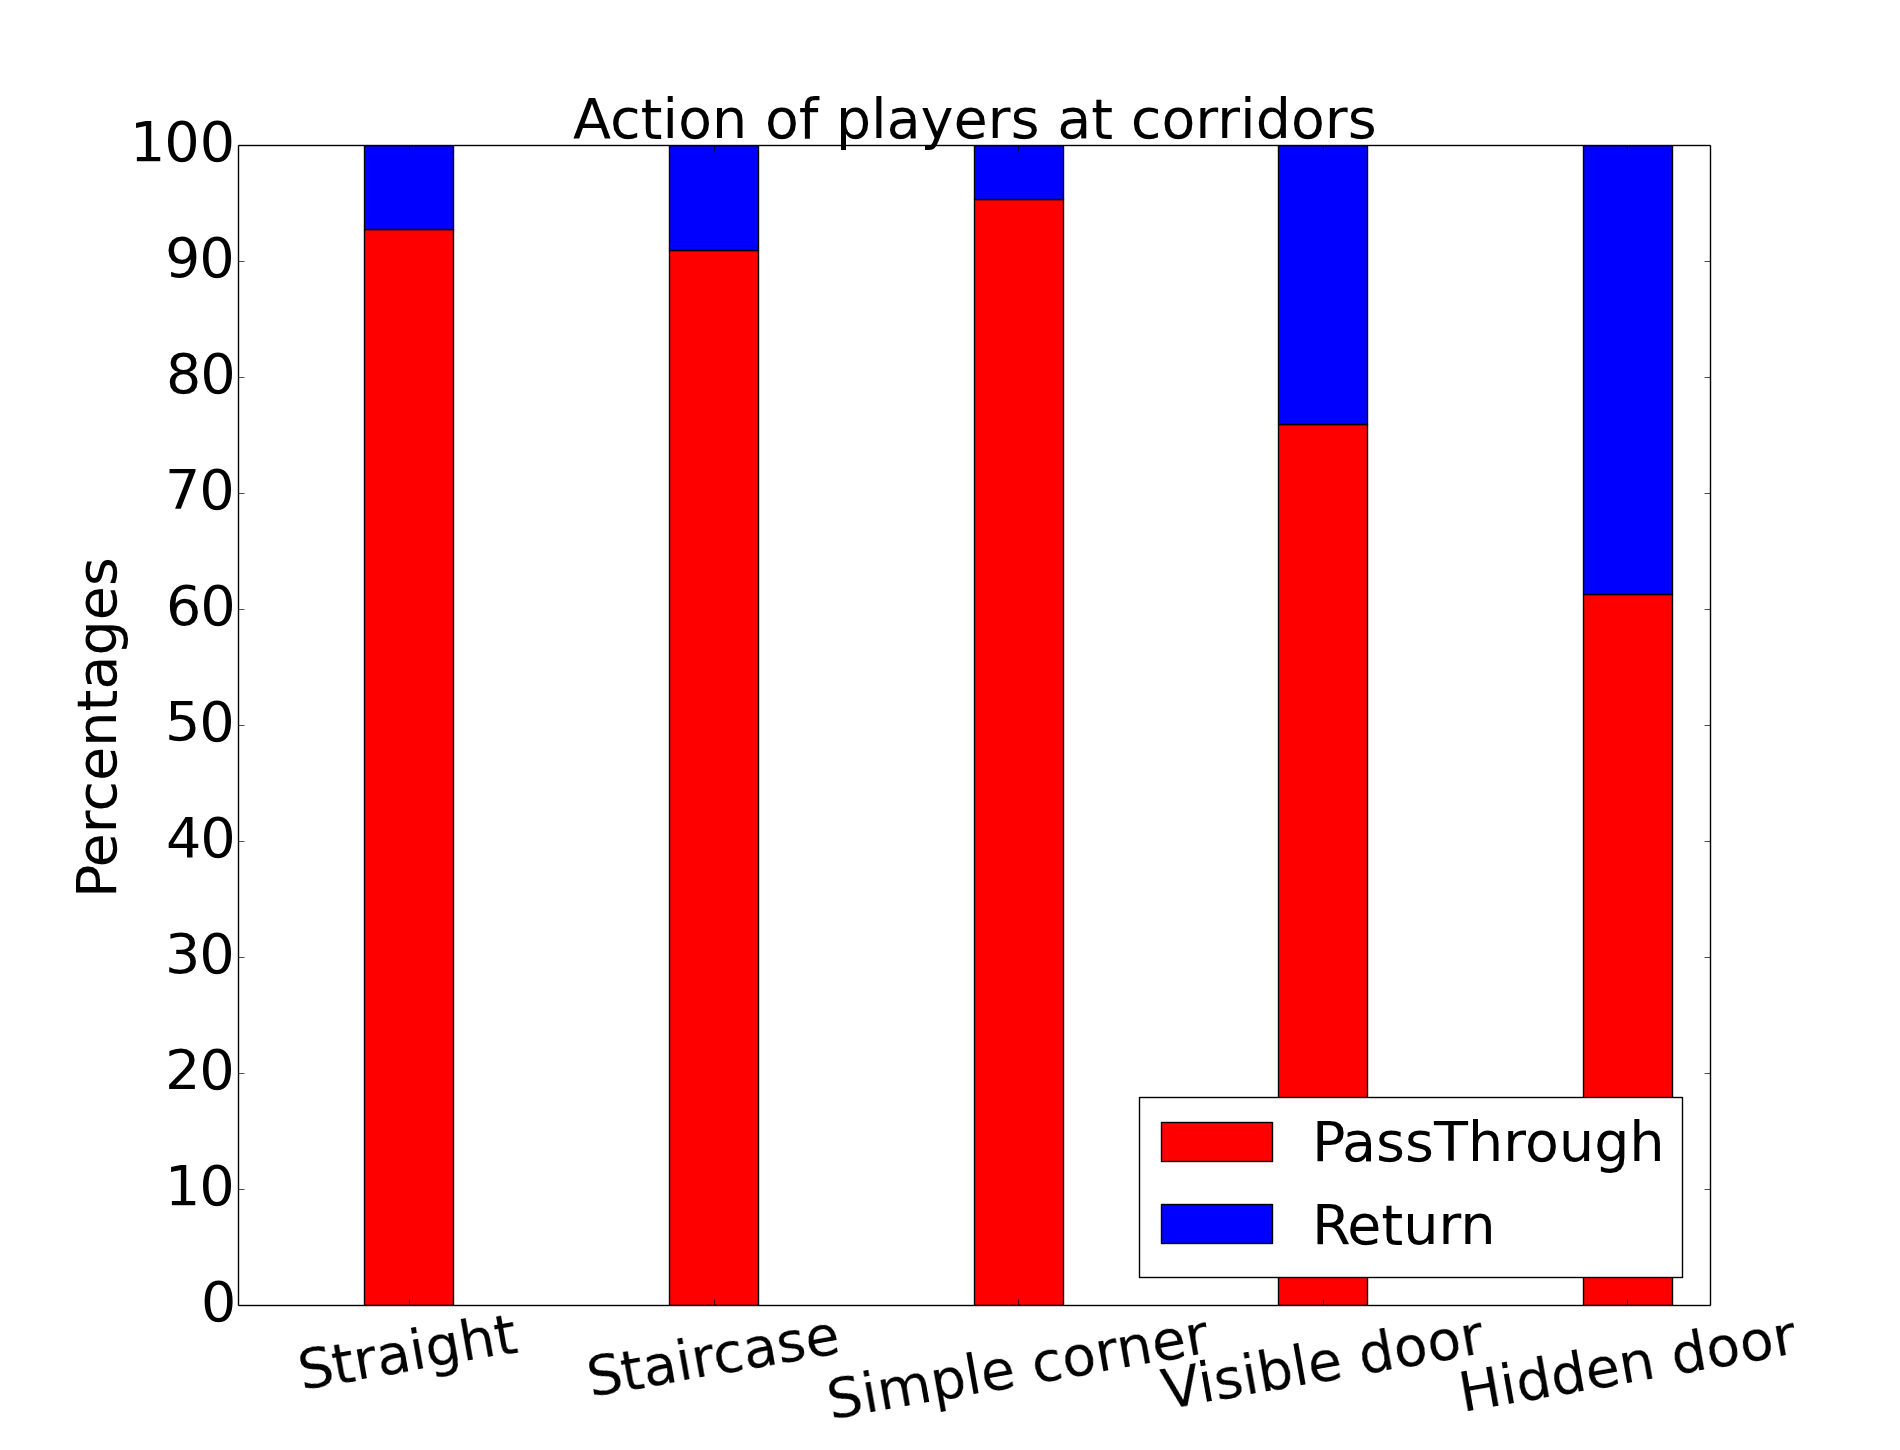
\includegraphics[width=\columnwidth]{SpatialKnowledge/simpleCorridorBehavior.png}
    \end{center}
    \caption[Existence of definite decision points]{This chart summarizes the behavior at corridors of different types. Less than $10\%$ of the players make a conscious decision (i.e. change their direction) on a straight corridor, a staircase, or even a simple corner. More interestingly, a little less than $25\%$ go back instead of opening a clearly visible door in front of them. However, when this next door is not clearly visible when they enter, there is $40\%$ of the player just going back through their entrance. This indicates that there are definite decision points during exploration.}
    \label{fig:simpleCorridorBehavior}
\end{figure}

Figure~\ref{fig:simpleCorridorBehavior} illustrates the decisions of people at different types of rooms and corridors, where it is possible for them to make a decision. At certain locations, such as corridors that have no rooms on the side (that is, they are simply connections between two areas), staircases and simple corners, the only decision that a player can make is whether to move forward or turn back. Turning back would require a conscious decision by the player. A pure random walker would generally have an equal chance of going back or forward. As shown in figure~\ref{fig:simpleCorridorBehavior}, the data reveals that players generally don't change their mind.

What is more interesting is the behavior of people at rooms which have just two doors. The data seems to reveal that if the opposite door is clearly visible from one door, then the room is used by the player almost exactly like a corridor, though there is a slightly higher chance of turning back than in a corridor. However, if the opposite door is not clearly visible when the person enters i.e. it is at some angle to the view when the player enters or there is some furniture partially blocking the view to that door, then there is more than $40\%$ chance of the person simply going back.

There is an argument to be made that this reluctance to move towards a slightly less visible door is a result of the input controls (keyboard and mouse) of the game. However, we believe this is not the case because we believe the data that was used consists of players who did not find it difficult to turn. We believe this because only the data of players who managed to complete the game within the time limit was included. As doing this required exploring a complicated 3 floor environment with 44 rooms and plenty of turns, the players had to be able to use the movement and turning controls in a reliable and natural manner.



% section definite_decision_points (end)

\subsubsection{Location recognition and memory} % (fold)
\label{sec:on_memory_and_exploration}

\begin{figure}[!tb]
    \begin{center}
        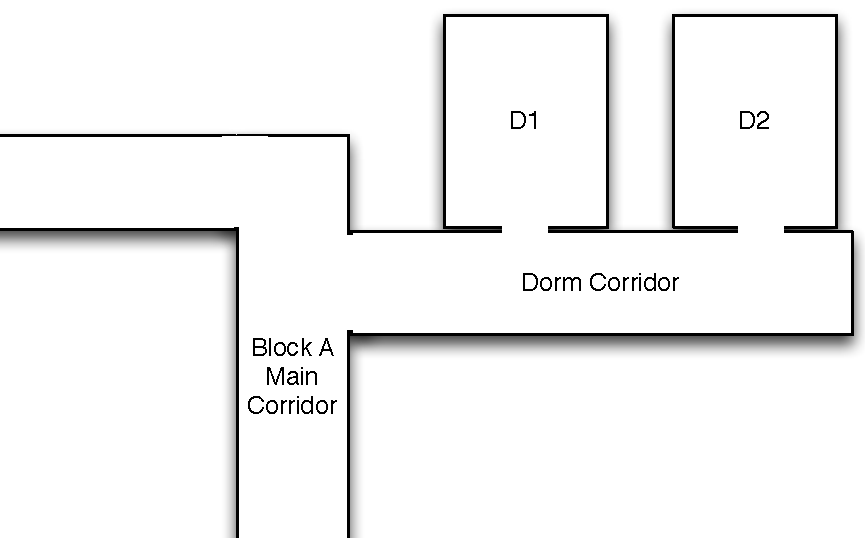
\includegraphics[]{SpatialKnowledge/dormCorrLayout}
    \end{center}
    \caption[Layout of dorm corridor]{The layout of the area under consideration for analysing location recognition and memory.}
    \label{fig:dormCorrLayout}
\end{figure}

In the game environment, there exists a corridor that seems to reveal an interesting aspect of memory and exploration. The layout of this corridor is shown in Figure~\ref{fig:dormCorrLayout}. The corridor labeled \emph{Dorm Corridor} is interesting because it is connected to the main Block A corridor only at one end. The two rooms on this corridor (D1 and D2) do not have a prison, a staircase, or any connections that make it at all relevant to the player. However, it lies on a commonly used corridor (marked Block A Main Corridor) and is used by most players at least once. In an ideal scenario, players would remember this fact and never visit \emph{Dorm Corridor} after the first visit to the junction of \emph{Block A Main Corridor} and \emph{Dorm Corridor}. The actual movement of the players at this junction is shown in Figure~\ref{fig:junctionA2Behavior}. Surprisingly, the figure shows that during the task completion phase, regardless of the number of times the junction is visited during exploration (on average around 2-7 times per player), players almost always turn into the \emph{Dorm Corridor}.

\begin{figure}[!tb]
    \begin{center}
        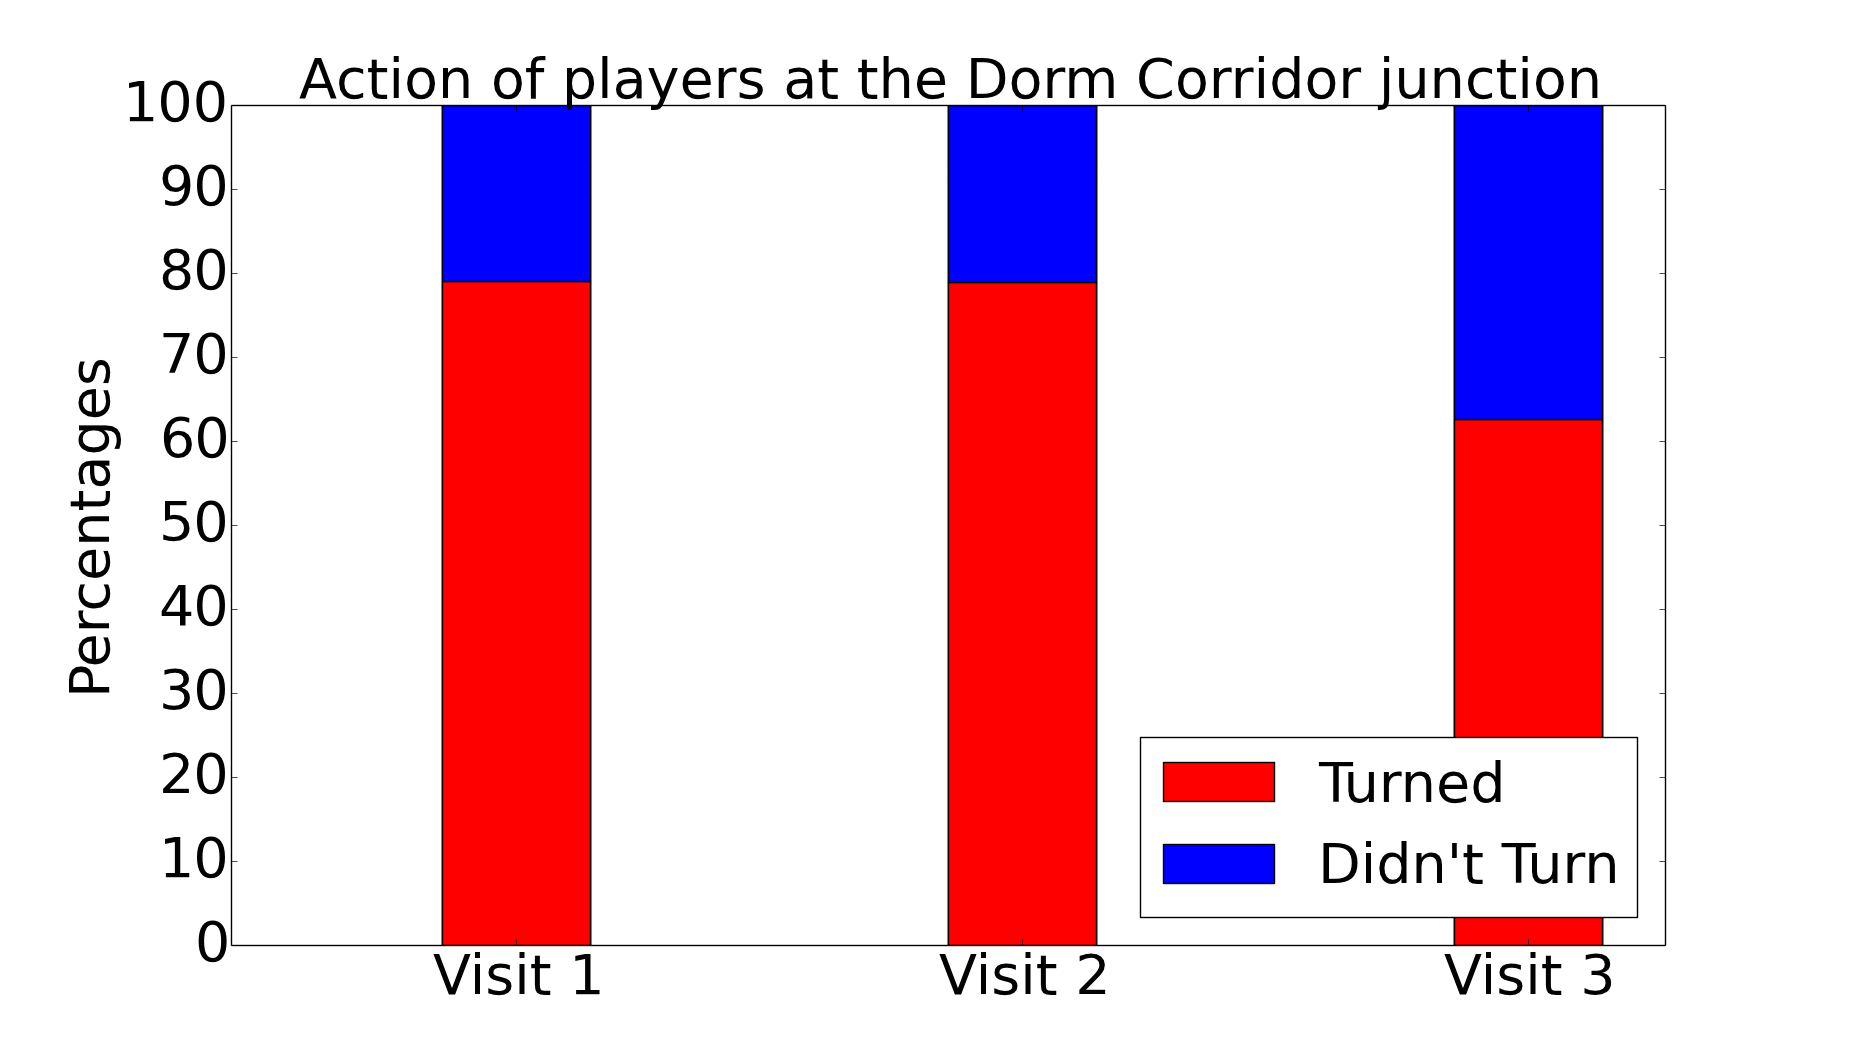
\includegraphics[width=\textwidth]{SpatialKnowledge/CorrA2-tasks.png}
    \end{center}
    \caption[Player behavior at junction under consideration]{This figure shows the movement of the players at the junction of Block A Main Corridor and the Dorm Corridor  during the Knowledge Testing Phase. As can be clearly seen, players keep revisiting the corridor despite having visited it before}
    \label{fig:junctionA2Behavior}
\end{figure}
\begin{figure}[!tb]
    \begin{center}
        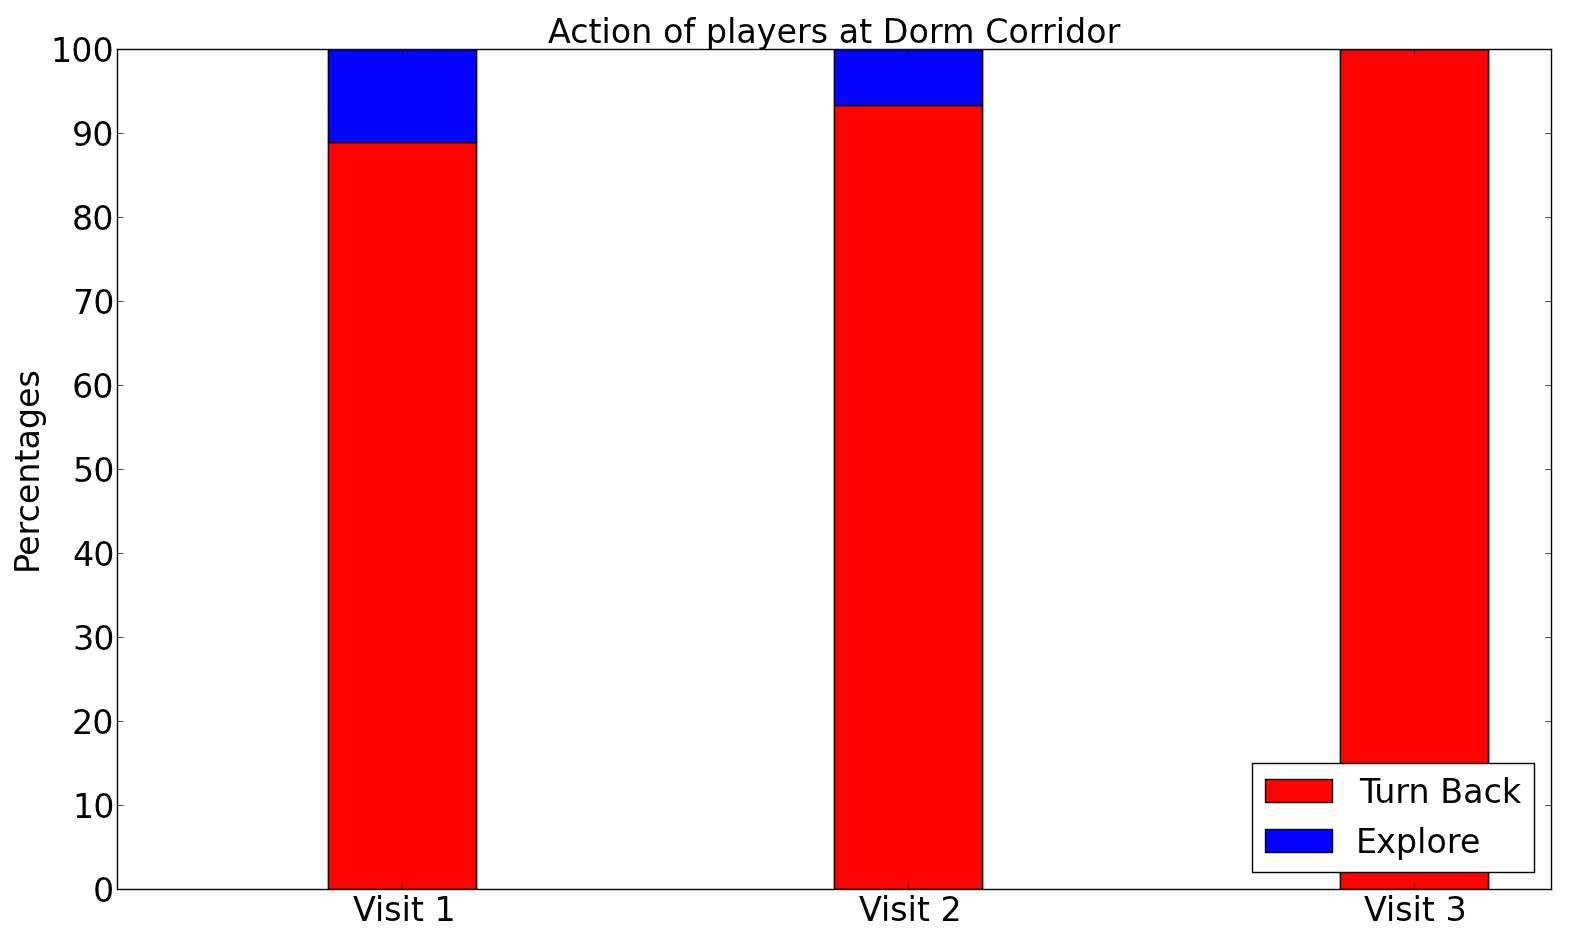
\includegraphics[width=\textwidth]{SpatialKnowledge/DormCorr-tasks.png}
    \end{center}
    \caption[Player behavior at dorm corridor]{This figure shows the behavior of the players after entering \emph{Dorm Corridor} during  the Knowledge Testing Phase. At this point, most players remember the corridor and head back to the Main Corridor without exploring}
    \label{fig:dormCorrBehavior}
\end{figure}

At first this leads to the conclusion that the players never learn and have no memory. However, a similar analysis of movement after entering \emph{Dorm Corridor} indicates that this isn't the case. As shown in Figure~\ref{fig:dormCorrBehavior} about $80\%$ of the players head right back to the junction after entering this corridor. This probably indicates that the context given by the location of signs and doors in the corridor helps the player remember the corridor, its location and its use.



% section empiricalanalysis (end)


% section replicating_the_exploration_behavior (end)

\section{Conclusion and Future Work} % (fold)
\label{sec:conclusion}

In this chapter, we presented a novel game-based methodology that allows for experimental investigation of human navigation and exploration. Although similar methodologies have been used to understand more general crowd behavior, we believe this is the first case in which quantitative analysis of a game has been used to understand the role memory plays in exploration. The novel Markovian analysis of the player's movement in the game revealed a number of significant findings. Firstly, we showed that a simple memory model, with a depth of between 6-8, is sufficient to approximate a `human level' of exploration efficiency. This was consistent in two measures of exploration efficiency: total coverage from a fixed number of hops and the number of hops required to obtain a fixed coverage. The memory depth of 6-8 seems to be consistent with well known studies of human memory capacity. The experiments also highlighted the importance of junctions in the exploration process, in particular, decisions (that is, changing course) seem to almost exclusively occur at junctions. Explorers also try to reduce the number of decisions they have to make by proceeding to the next clearly visible room or corridor (assuming only one such room is visible). Furthermore, the results showed that people seem to explore environments using a floor first strategy, where they are reluctant to move to a different floor until they have finished exploring the current one. Finally, we show that easily recognizable locations probably help individuals improve exploration efficiency by enabling individuals to effectively remove sub-graphs of the room network from their cognitive map.

Several of these observations could be made only through the analysis of the movement graphs and the Markovian analysis on the data. It would have been difficult to obtain this amount of data through the traditional experimental methodologies without significant cost in terms of time and effort. Thus, a game based analysis is not only useful in making significant observations about human behavior but in also helps open up new possibilities of research.

The simple agent-based memory model developed in the paper is shown to approximate human-like efficiency in its exploration strategy. We think this type of model is an excellent starting point for developing agent-based models that can be used to evaluate safety-by-design architecture in complex structures. We also see the experiments and methods presented here as a starting point for further investigations into the role of exploration and memory in human egress. Similar experiments could be conducted to evaluate the role of long-term memory in exploration, and perhaps validate the three-stage map building of Siegel and White~\cite{Siegel19759}.



% section comparison_and_final_discussion (end)


\subsection{Future Work: Scaling The Game} % (fold)
\label{sec:scaling_the_game}

Section~\ref{sec:analysis_of_experiment_results} analyzed the result of fifty students playing the game. One of the limitations of the analysis discussed in this chapter was the amount of data that was available for analysis especially for the Markov analysis. The limited number of participants available also meant that it was difficult to test hypothesis on the task completion phase by creating and comparing the players movement in an alternate environment.

As discussed in Section~\ref{sec:the_minecraft_gaming_environment}, one of the big advantages of using a popular game like Minecraft with over 35 million copies sold, is the ubiquity of the game. To make use of this ubiquity, we have hosted the game on a Linux Server provided by Amazon Web Services and plan to collect data from this server over the next year. First a simple web page (\url{vaisaghvt.com/minecraft-experiment/}) was created where interested players can submit a request to play by using a registered Minecraft account. This request is sent to the Amazon Server. Python's event driven network engine \emph{Twisted}~\cite{TwistedLink} was used to create a simple application that listens to these requests at a specified port and starts a white-listed Minecraft Server to which only this particular user can connect. Once a request is successful, the player receives the IP address of the machine which he proceeds to use to connect to the server and play the game. The Minecraft Server is shut down once the player exits the game.

Due to the cost of running a virtual server with 3 GB memory, we have only one server and thus only one player is able to connect at any given time. With about 1-3 players a day, we hope to collect data from 500-1000 players over the next year. This much greater sample will hopefully reveal more fundamental and interesting aspects of human exploration behavior than was possible to analyze with the limited dataset currently available. The setup of the experiment also makes it relatively easy to scale to multiple servers if they are available. Running different experiments just involves replacing a single folder with a different setup. With enough data, this can be used to do A/B testing to test different hypothesis.

